% This is a LaTeX thesis template for Monash University.
% to be used with Rmarkdown
% This template was produced by Rob Hyndman
% Version: 6 September 2016

\documentclass{monashthesis}

%%%%%%%%%%%%%%%%%%%%%%%%%%%%%%%%%%%%%%%%%%%%%%%%%%%%%%%%%%%%%%%
% Add any LaTeX packages and other preamble here if required
%%%%%%%%%%%%%%%%%%%%%%%%%%%%%%%%%%%%%%%%%%%%%%%%%%%%%%%%%%%%%%%

\author{Nicholas S Spyrison}
\title{Dynamic visualization of high-dimensional data via low-dimension
projections and sectioning across 2D and 3D display devices}
\degrees{B.Sc. Statistics, Iowa State University}
\def\degreetitle{Doctor of Philosophy}
% Add subject and keywords below
\hypersetup{
     %pdfsubject={The Subject},
     %pdfkeywords={Some Keywords},
     pdfauthor={Nicholas S Spyrison},
     pdftitle={Dynamic visualization of high-dimensional data via low-dimension
projections and sectioning across 2D and 3D display devices},
     pdfproducer={Bookdown with LaTeX}
}


\bibliography{thesisrefs}

\begin{document}

\pagenumbering{roman}

\titlepage

{\setstretch{1.2}\sf\tighttoc\doublespacing}

\chapter*{Abstract}\label{abstract}
\addcontentsline{toc}{chapter}{Abstract}

Visualizing data space is crucial to exploratory and general data
analysis yet doing so quickly becomes difficult as the dimensionality of
the data increases. Traditionally, static, low-dimensional linear
embeddings are used to identify clustering, outliers, and structure.
Observing one such embedding often misses a significant amount of
variation, and hence, information held within the data. \emph{Tours} are
a class of dynamic linear projections that animates many linear
projections as the orientation in data space changes. This maintains
transparency to the original variables while preserving information in
the data. User-controlled steering (UCS) of the original dimensionality
offers fine control of the local structure of projections.

Data visualization has lagged behind in implementing 3D and virtual
spaces after, overhype and excitement from the 1980s and '90s. Modern
mixed reality hardware has significantly improved the quality and
simultaniously reduced the barrier to entry. Contemporary studies have
regularly shown increased accuracy of perception of visuals displayed in
3D over 2D, including in projected subspaces. It's time to further
explore dynamic projections in virtuals spaces

Multivariate data is ubiquitous and viewing it in data-space is a
crucial aspect of data analysis and consumption. This research allows
for fine exploration of the data structure in embeddings of high
dimensional spaces, contrasts UCS with traditional static techniques,
implements known and surface dynamic projections in 3D space, and
quantifies the benefits of dynamic projections across display types.

\clearpage\pagenumbering{arabic}\setcounter{page}{0}

\chapter{Introduction}\label{ch:introduction}

\section{Exploratory data analysis}\label{exploratory-data-analysis}

The term exploratory data analysis was coined in
\textcite{tukey_exploratory_1977}. Tukey does not specify specific
processes and uses the term to encompass more broad aspects to initial
summarization and visualization. This is the first conceptualization of
the structure of the data and should validate assumptions made by
prospective methodology. Visualization is crucial to a clear
understanding of the data. Things can go awry when data is summarized
via numeric statistics alone \autocite{anscombe_graphs_1973},
demonstrated in figure \ref{fig:matejka17fig}
\autocite{matejka_same_2017}. In these studies, bivariate data have the
same summary statistics, such as mean and standard deviation, yet
contain obvious visual trends and shapes that could go completely
unheeded if graphing the data is foregone. Because there are inherent
dangers to relying on statistics alone, this requirement for looking at
visuals necessitates \emph{human-in-the-loop} analysis, defined as a
model that requires human interaction.






\begin{figure}

{\centering 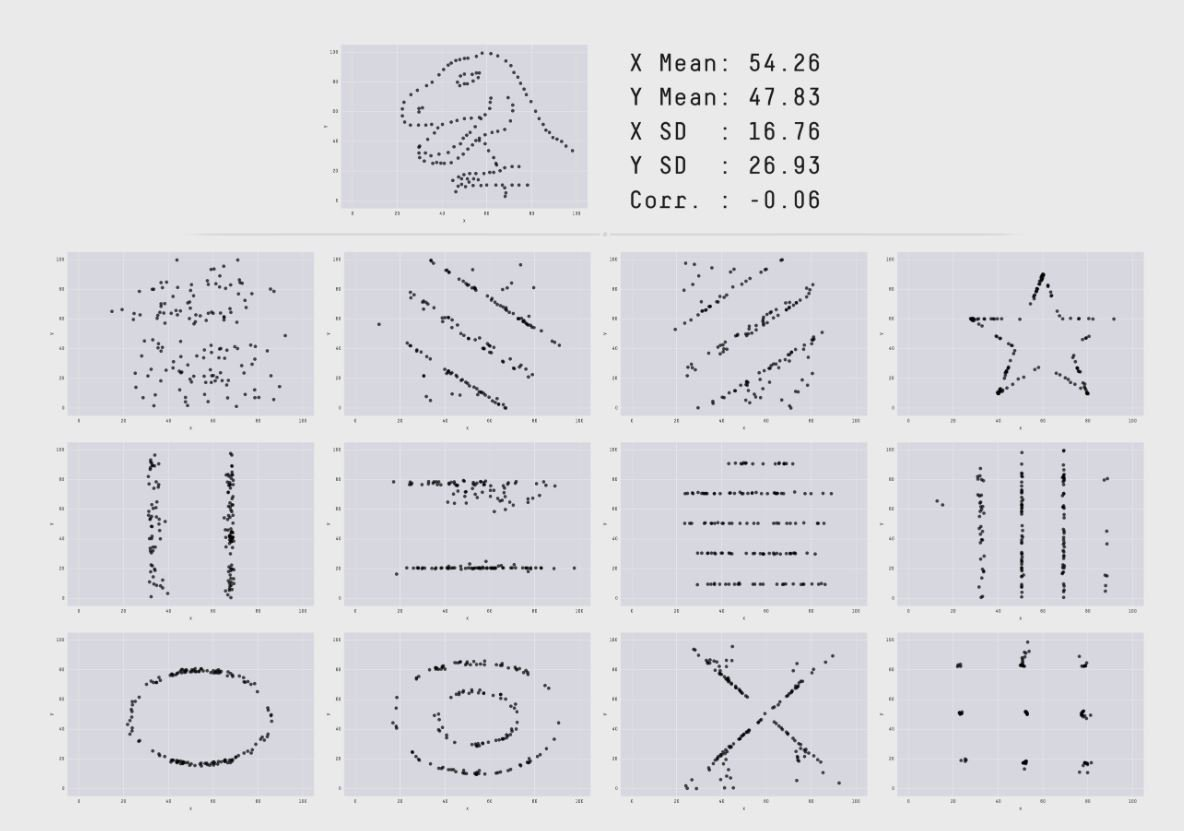
\includegraphics[width=0.7\linewidth]{./figures/matejka17fig} 

}

\caption{12 data sets created from the datasaurus by
simulated annealing. Each is restrained to the same summary statistics
but given shapes with visual peculiarity to mutate into
\autocite{matejka_same_2017}.}\label{fig:matejka17fig}
\end{figure}

It is clear that data-space visualization is needed but becomes complex
as data dimensionality increases. Embedding (or projecting)
\(p-\)dimensional data on to a lower, \(d\)-dimensional subspace is a
common dimension reduction approach to visualize multivariate data
spaces. Traditionally a single static projection is used to summarize a
space, which necessarily shows a subset of the variation of the data.
\textcite{asimov_grand_1985} suggested the use of viewing projections
dynamically across a changing projection basis allows for more variation
to be contained and viewed temporally. This dynamic view of many
changing projections is known as \emph{tours}. While, there are
different methods of generating tour paths, human-in-the-loop
user-controlled steering (UCS) offers the finest control for navigating
the local structure and is particularly useful in exploration after an
interesting feature has been identified.

Tours commonly view \(d=\{1, 2, 3\}\) embedded subspaces from standard
2D monitors, and most commonly viewed as a projection down to 2D. The
exception being \textcite{nelson_xgobi_1998}, where 3D tours were viewed
in 3D head-tracked VR. Data visualization studies generally show an
improved perception of 3D visuals over 2D, especially when adequate
depth cues are provided. The state of modern hardware improvements has
made VR more affordable and available to wider audiences, at ever
increasing resolutions of display than previously possible. Research
should be conducted to compare the perception of dynamic linear
projections across display type.

\section{Research objectives}\label{research-objectives}

Data and models are typically high-dimensional, with many variables or
parameters. Developing new methods to visualize high dimensions has been
a pursuit of statisticians, computer scientists and visualization
researchers for decades. As technology evolves examining, extending, and
assessing current techniques, in new environments, for new data
challenges, is an important endeavor. The primary goal of this
Ph.D.~research can then be summarized as:

\textbf{Research objectives (RO):}

\begin{enumerate}
\def\labelenumi{\arabic{enumi}.}
\tightlist
\item
  \textbf{How can UCS be implemented in 1- and 2D projections?} (Work in
  progress, chapter \ref{ch:workinprogress}.) Following the theory laid
  out in \textcite{cook_manual_1997}, a new UCS algorithm is devised for
  use in animation specific implementations. This enables fine control
  of exploring the local structure of data in 2D embeddings, setting a
  framework to be used in the remaining objectives.
\item
  \textbf{Does 2D UCS provide benefits over alternatives?} (Future work,
  chapter \ref{ch:future_work}.) The quality and effectiveness of the
  dynamic UCS will be compared to benchmark datasets against commonly
  used alternatives of static, single, linear and non-linear projection
  techniques. The addition of the temporal dimension theoretically
  allows for more information to be conveyed than in static projections.
\item
  \textbf{How can UCS be extended to 3D?} (Future work, chapter
  \ref{ch:future_work}.) The UCS algorithm needs to be extended to a
  third dimension and the rendering of 3D dynamic projections and
  sectioning for use across mixed reality display devices.
\item
  \textbf{Does UCS in 3D displays provide perception benefits over 2D
  displays?} (Future work, chapter \ref{ch:future_work}.) The addition
  of a stereoscopic 3rd dimension has previously shown improved
  perception in other visualization. Building on the work from the
  previous objective the efficacy of 3D tours should be explored using
  modern hardware across display devices (including 2D standard monitor,
  3D head tracked monitor, and 3D head-mounted display).
\end{enumerate}

\section{Methodology}\label{methodology}

This research is interdisciplinary; it's base on a dimension reduction
technique developed by statisticians, extended with information
technology into 3D including VR technologies, with applications in high
energy physics identified\autocite{cook_dynamical_2018}. The research is
correspondingly supervised experts in these fields.

The research corresponding with RO \#1 entails a work in progress
\textbf{algorithm design} following the work in
\textcite{cook_manual_1997} to allow for UCS. The proposed algorithm
discusses the generalized application of UCS for use across animation
implementations. This outcome of this is an \emph{R} package,
\texttt{spinifex}, which will be submitted to CRAN and for hosting and
distribution. This forms the foundation for future work in the remaining
objectives.

The second objective is addressed with a benchmark dataset comparison
\textbf{case study} between dynamic linear projections and alternatives
(static linear and static non-linear projections such as Principal
Component Analysis, Multi-Dimensional Scaling, and t-distributed
neighbor embeddings, described in more detail in chapter
\ref{ch:future_work}). Benchmark datasets will be compared across
techniques, measurements will include variation explained, transparency
to the original variable space, clustering, and outlier identification.

The research for RO \#3 involves \textbf{algorithm design}, where the
work in RO \#1 will be extended to the third dimension. Surface and
function projections will also be developed. This forms the calculation
base for the work. Several difficulties may arise in bringing dynamic
touring to 3D spaces, especially when exploring 3D surfaces (discussed
in more detail in chapter \ref{ch:future_work}).

The research resulting from RO \#4 is a controlled \textbf{usability
study} to explore the efficacy of bringing UCS into 3D as compared
across various display devices, in a standardized interface allowed by
the work stemming from RO \# 3. In this design, every participant will
complete every task on every display device. Quantitative measurements
include participant speed and accuracy of tasks, biometric readings, and
subjective Likert surveys of participants. A lineup-type model as
outlined in \textcite{hofmann_graphical_2012} may also be employed for
assessing the quality of display types.

\section{Workflow and
reproducibility}\label{workflow-and-reproducibility}

Figure \ref{fig:dataanalysisworkflow} depicts the general data analysis
workflow \autocite{wickham_r_2016}. Where data first must be imported
into a tool, the structure of the data must be tidied and ordered neatly
into the correct use format. After the data enters a repeating cycle,
where values may be transformed, visualized, and modeled with
communication going to the appropriate recipients. The research proposed
in this document aids exploratory data analysis as well as the
visualization aspect of this workflow. Mature analysis workflow is also
made reproducible with the use of programmatic scripts.





\begin{figure}

{\centering 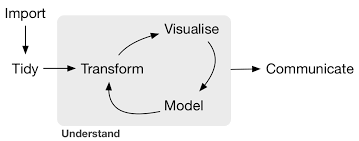
\includegraphics[width=1\linewidth]{./figures/data_analysis_workflow} 

}

\caption{Data analysis workflow
\autocite{wickham_r_2016}. This research aids visualization in
exploratory data analysis and workflow.}\label{fig:dataanalysisworkflow}
\end{figure}

The programing language, \emph{R}, is used in the work described below
to import, tidy, and transform data. It can be used directly to
visualize 2D tours (RO \#1 \& 2) or be consumed into the game engine
\emph{Unity} to visualize 3D tours (RO \#3 \& 4). Doing analysis and
writeup in such programmatic ways allow work to be done reproducibly.
Where data, analysis, and code are stored in the same directory.
Reproducible work facilitates validation, maintains transparency and
minimizes the chance for human error. Reproduction of work is a key
feature to validate and defend the claims and methodology held within a
work. Directories of current and planned work are/will be hosted
publicly on GitHub, including this report. Accessing the source files
for this report is discussed in section \ref{sec:source}.

\section{Project overview}\label{ch:projectoverview}

The research gaps in the literature review leave room for the research
objectives outlined in the introduction. Figure
\ref{fig:ProjectOverview} depicts a schematic flow chart that the
research objectives will be executed in. The research responding to RO
\#1, the application of 2D user-controlled steering (UCS), sets the
foundation for which the other objectives can be researched. RO \#3, the
application of 3D UCS, must precede RO \#4, exploring the efficacy of 3D
UCS across display devices. RO \#2, the comparison of 2D UCS vs
alternatives, must come after RO \#1, but is of lower priority to RO \#3
\& 4, and so will be conducted last, in the event of a time crunch.




\begin{figure}

{\centering 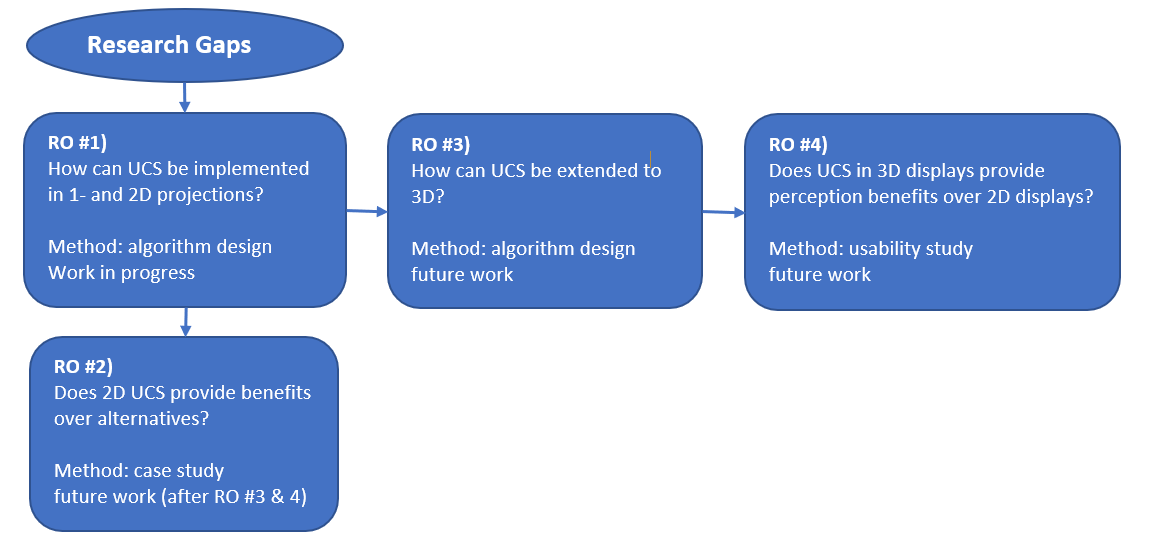
\includegraphics[width=1\linewidth]{./figures/ProjectOverview} 

}

\caption{Flow chart of research objective dependencies,
work order, and methodology.}\label{fig:ProjectOverview}
\end{figure}

In this report, the related literature is discussed in chapter
\ref{ch:lit_review}. A brief overview of the research is given in
chapter \ref{ch:projectoverview}, followed by ongoing work and future
work in chapters \ref{ch:workinprogress} and \ref{ch:future_work}
respectively. A prospective timeline is listed in chapter
\ref{ch:timeline}. Notation for dynamic touring and VR data
visualization can be found in appendix \ref{ch:glossary}, and an excerpt
of a paper to be submitted to the R Journal can be found in appendix
\ref{ch:spinifex_paper}.

\chapter{Literature review}\label{ch:lit_review}

In the following chapter, we discuss the current research in two primary
areas: dynamic linear projection (collectively known as tours) and
multivariate data visualization in stereoscopic 3D. After each section,
we highlight the research gaps and show how they relate to the research
objectives.

\section{Dynamic linear projections of multivariate data
(tours)}\label{sec:tour}

\subsection{Overview}\label{overview}

The introduction established that visualizing data-space is an important
aspect of exploratory data analysis and data analysis in general. Yet,
there is an inherent difficulty as the dimensionality of data increases.
In univariate data sets histograms or smoothed density curves are
employed to visualize data. In bivariate data, \(x-y\) scatterplots and
contour plots (2D density) can be employed. In three dimensions the two
most common techniques are 3D
scatterplot\footnote{Graphs depicting three dimensions are typically viewed on a 2D display, in print or with a standard monitor. These are 2D images of monocular 3D spaces, sometimes referred to as 2.5D data visualization, more on this in section \ref{sec:3d-terminology}.}
or 2D scatterplot with the 3rd variable as an aesthetic (such as color,
size, or height). These aesthetic cues convey some information but are
not a sufficient replacement for axes for use with continuous variables.

As dimensionality of the data, \(p\), increases the visualization of
data-space quickly becomes complex. It's common that visualizing
data-space is dropped in favor of graphing model-space (for example
residuals), parameter-space (in fewer dimensions), or worse yet: long
tables of statistics without visuals
\autocite{wickham_visualizing_2015}. To preserve the visualization of
data-space, a solution that scales with the dimensionality of data is
needed; this is where dimensionality reduction comes in. This work will
focus on a group of dynamic linear projection techniques collectively
known as \emph{tours}. A broader review of dimensionality reduction
techniques is discussed in \textcite{grinstein_high-dimensional_2002},
and \textcite{heer_tour_2010}. Tours are used for a couple of salient
features: the use of linear projections maintains transparency back to
the original variable space (which non-linear projections lose) and
views many projections showing more variation than a single linear
projection could show. Employing the breadth of tours extends the
dimensionality of visualizations, and with it, the intrinsic
understanding of the structure and distribution of data that is more
succinct or beyond the reach of summary statistics alone.

Let \(p\) be the dimensionality of the data, and \(d\) be the dimension
of the projection space. Tours perform linear dimensionality reduction,
orthogonally projecting \(p\)-space down to \(d(\leq p)\) dimensions.
Many such projections are interpolated, each making small rotations in
\(p\)-space. These frames are then viewed in order as an animation of
the lower dimensional embedding changing as the original variable space
is manipulated. Shadow puppets offer a useful analogy to aid in
conceptualizing touring. Imagine a fixed light source facing a wall.
When an object is introduced it projects a 2D shadow onto the wall. This
is a physical representation of a simple projection, that from \(p=3\)
down to \(d=2\). If the object rotates then the shadow correspondingly
changes. Observers watching only the shadow are functionally watching a
2D tour as the 3D object is manipulated. Some orientations explain more
information about the shape of the object than others but watching an
animation of the shadow changing gives a more robust understanding than
looking at any one frame. More complex structures generally require more
time to comprehend the nature of the geometry. These features hold in
touring as well.

\emph{Tour notation is listed in the appendix section
\ref{sec:tour_notation}.}

\subsection{History}\label{history}

Touring was first introduced by \textcite{asimov_grand_1985} with his
purposed \emph{grand tour} at the Stanford Linear Accelerator, Stanford
University. In which, Asimov suggested three types of grand tours:
torus, at-random, and random-walk. The original application of tours was
performed on high energy physics on the PRIM-9 system.

Before choosing projection paths randomly, an exhaustive search of
\(p-\)space was suggested by \textcite{mcdonald_interactive_1982}, also
at the Stanford Linear Accelerator. This was later coined \emph{little
tour}.

\textcite{friedman_projection_1974} and later
\textcite{huber_projection_1985} recommended projection pursuit (also
referred to as PP). Projection pursuit involves identifying
``interesting'' projection, remove a single component of the data, and
then iterates in this newly embedded subspace. Within each subspace, the
projection seeks for a local extremum via a hill climbing algorithm on
an objective function. This formed the basis for \emph{guided tours}
suggested by \textcite{hurley_analyzing_1990}.

The grand and little tours have no input from the user aside from the
starting basis. Guided tours allow for an index to be selected, but the
bulk of touring development since has largely been around the dynamic
display, user interaction, geometric representation, and application.
The details are expounded on in the following sections.

\subsection{Path generation}\label{sec:path_generation}

A fundamental aspect of touring is the path of rotation. Of which there
are four primary distinctions \autocite{buja_computational_2005}: random
choice, data-driven, precomputed choice, and manual control.

\begin{itemize}
\tightlist
\item
  Random choice, \emph{grand tour}, constrained random walks
  \(p\)-space. Paths are constrained for changes in direction small
  enough to maintain continuity and aid in user comprehension

  \begin{itemize}
  \tightlist
  \item
    torus-surface \autocite{asimov_grand_1985}
  \item
    at-random \autocite{asimov_grand_1985}
  \item
    random-walk \autocite{asimov_grand_1985}
  \item
    \emph{local tour} \autocite{wickham_tourr_2011}, a sort of grand
    tour on a leash, such that it goes to a nearby random projection
    before returning to the original position and iterating to a new
    nearby projection.
  \end{itemize}
\item
  data-driven, \emph{guided tour}, optimizing some objective
  function/index within the projection-space, called projection pursuit
  (PP) \autocite{hurley_analyzing_1990}, including the following
  indexes:

  \begin{itemize}
  \tightlist
  \item
    holes \autocite{cook_projection_1993} - moves points away from the
    center.
  \item
    cmass \autocite{cook_projection_1993} - moves points toward the
    center.
  \item
    lda \autocite{lee_projection_2005} - linear discriminant analysis,
    seeks a projection where 2 or more classes are most separated.
  \item
    pda \autocite{lee_projection_2010} - penalized discriminant analysis
    for use in highly correlated variables when classification is
    needed.
  \item
    convex \autocite{laa_using_2019} - the ratio of the area of convex
    and alpha hulls.
  \item
    skinny \autocite{laa_using_2019} - the ratio of the perimeter
    distance to the area of the alpha hull.
  \item
    stringy \autocite{laa_using_2019} - based on the minimum spanning
    tree (MST), the diameter of the MST over the length of the MST.
  \item
    dcor2D \autocites{grimm_mbgraphic:_2017}{laa_using_2019} - distance
    correlation that finds linear and non-linear dependencies between
    variables.
  \item
    splines2D \autocites{grimm_mbgraphic:_2017}{laa_using_2019} -
    measure of non-linear dependence by fitting spline models.
  \item
    other user-defined objective function can be implemented with the
    \emph{tourr} package \textcite{wickham_tourr_2011}.
  \end{itemize}
\item
  Precomputed choice, \emph{planned tour}, in which the path has already
  been generated or defined.

  \begin{itemize}
  \tightlist
  \item
    \emph{little tour} \autocite{mcdonald_interactive_1982}, where every
    permutation of variables is stepped through in order, analogous to
    brute-force or exhaustive search.
  \item
    a saved path of any other tour, typically an array of basis targets
    to interpolate between.
  \end{itemize}
\item
  Manual control, \emph{manual tour}, a constrained rotation on selected
  manipulation variable and magnitude \autocite{cook_manual_1997}.
  Typically used to explore the local area after identifying an
  interesting feature, perhaps via guided tour.
\item
  \emph{dependence tour}, a combination of \(n\) independent 1D tours. A
  vector describes the axis each variable will be displayed on. for
  example \(c(1, 1, 2, 2)\) is a 4- to 2D tour with the first 2
  variables on the first axis, and the remaining on the second.

  \begin{itemize}
  \tightlist
  \item
    \emph{correlation tour} \autocite{buja_data_1987}, a special case of
    the dependence tour, analogous to canonical correlation analysis.
  \end{itemize}
\end{itemize}

\subsection{Path evaluation}\label{path-evaluation}

Consider projection to 2D, then each projection is called a 2-frame
(each spanning a 2-plane). Mathematically, a Grassmannian is the set of
all possible unoriented 2-frames in \(p\)-space, \(\textbf{Gr}(2,~p)\).
\textcite{asimov_grand_1985} pointed out that the unique 2-frames of the
grand tour approaches \(\textbf{Gr}(2,~p)\) as time goes to infinity.
The \emph{density} of a tour is defined as the fraction of the
Grassmannian explored. Ideally, an exploring tour will be dense, but the
time taken to become dense vastly increases as variable space increases
dimensionality. \emph{Rapidity} is then defined as how quickly a tour
encompasses the Grassmannian. Due to the random selection of a grand
tour, it will end up visiting homomorphisms of previous 2-frames before
all unique values are visited, leading sub-optimal rapidity.

The little tour introduced in \textcite{mcdonald_interactive_1982}, on
the other hand, is necessarily both dense and rapid, performing
essentially an exhaustive search on the Grassmannian. However, this path
uninteresting and with long periods of similar projections strung
together. The Grassmannian is necessarily large and increases with the
square of \(p\). Viewing of the whole Grassmannian is time-consuming,
and interesting projections are sparse, there was a clear space for
computers to narrow the search space.

Guided tours \autocite{hurley_analyzing_1990} optimize an objective
function generating path will be a relatively small subset of the
Grassmannian. As such, density and rapidity are poor measures, however,
interesting projections are quickly identified. Recently,
\textcite{laa_using_2019}, compared projection pursuit indices with the
metrics: \emph{smoothness, squintability, flexibility, rotation
invariance} and \emph{speed}.

\subsection{Geometric display by dimensionality}\label{sec:geom_display}

Up to this point, this document has discussed 2D scatterplots, which
offer a logical display for viewing embeddings of high-dimensional point
clouds. However, other geometrics offer perfectly valid projections as
well.

\begin{itemize}
\tightlist
\item
  1D geometrics (geoms)

  \begin{itemize}
  \tightlist
  \item
    1D densities: such as histogram, average shifted histograms
    \autocite{scott_averaged_1985}, and kernel density
    \autocite{scott_incorporating_1995}.
  \item
    image (pixel): \autocite{wegman_pixel_2001}.
  \item
    time series: where multivariate values are independently lagged to
    view peak and trough alignment. Currently no package implementation,
    but use case is discussed in \autocite{cook_manual_1997}.
  \end{itemize}
\item
  2D geoms

  \begin{itemize}
  \tightlist
  \item
    2D density (available on GitHub at
    \url{https://github.com/nspyrison/tourr})
  \item
    \(x-y\) scatterplot
  \end{itemize}
\item
  3D geoms

  \begin{itemize}
  \tightlist
  \item
    Anaglyphs, sometimes called stereo, where red images are positioned
    for the left channel and cyan for the right when viewed with
    corresponding filter glasses give a perception of depth to the
    image.
  \item
    Depth, which gives depth cues via aesthetic mappings, most common
    size and/or color of data points.
  \end{itemize}
\item
  \(d\)-dimensional geoms

  \begin{itemize}
  \tightlist
  \item
    Andrews curves \autocite{andrews_plots_1972}, smoothed variant of
    parallel coordinate plots, discussed below.
  \item
    Chernoff faces \autocite{chernoff_use_1973}, variables linked to the
    size of facial features for rapid cursory like-ness comparison of
    observations.
  \item
    Parallel coordinate plots \autocite{ocagne_coordonnees_1885}, where
    any number of variables are plotted in parallel with observations
    linked to their corresponding variable value by polylines.
  \item
    Scatterplot matrix \autocite{becker_brushing_1987}, showing a
    triangle matrix of bivariate scatterplots with 1D density on the
    diagonal.
  \item
    Radial glyphs, radial variants of parallel coordinates including
    radar, spider, and star glyphs \autocite{siegel_surgical_1972}.
  \end{itemize}
\end{itemize}

\subsection{Tour software
implementations}\label{tour-software-implementations}

Tours have not yet been widely adopted, this is likely due in part, to
the fact that print and static .pdf output does not accommodate dynamic
viewing. Conceptual abstraction and technically density have also
hampered user growth. Due to small adoption and rapid advancement of
technology support and maintenance of such implementations give them a
particularly short life span. Despite the small user base, there have
been a fair number of tour implementations, including:

\begin{itemize}
\tightlist
\item
  spinifex
  \href{https://github.com/nspyrison/spinifex}{github.com/nspyrison/spinifex}
  -- R package, all platforms.
\item
  tourr \autocite{wickham_tourr_2011} -- R package, all platforms.
\item
  CyrstalVision \autocite{wegman_visual_2003} -- for Windows.
\item
  GGobi \autocite{swayne_ggobi:_2003} -- for Linux and Windows.
\item
  DAVIS \autocite{huh_davis:_2002} -- Java based, with GUI.
\item
  ORCA \autocite{sutherland_orca:_2000} -- Extensible toolkit build in
  Java.
\item
  VRGobi \autocite{nelson_xgobi_1998} -- for use with the C2, tours in
  stereoscopic 3D displays.
\item
  ExplorN \autocite{carr_explorn:_1996} -- for SGI Unix.
\item
  XGobi \autocite{swayne_xgobi:_1991} -- for Linux, Unix, and Windows
  (via emulation).
\item
  XLispStat \autocite{tierney_lisp-stat:_1990} -- for Unix and Windows.
\item
  Explor4 \autocite{carr_explor4:_1988} -- Four-dimensional data using
  stereo-ray glyphs.
\item
  Prim-9 \autocites{asimov_grand_1985}{fisherkeller_prim-9:_1974} -- on
  an internal operating system.
\end{itemize}

\subsection{Research gaps}\label{research-gaps}

Currently, no compiling software offers UCS (\textbf{RO \#1}). This
leaves the class of dynamic linear projections without the most precise,
fine-scale control of rotating \(p\)-space. This should be reimplemented
with an eye on extensibility and maintainability,

A comparative study outlining the benefits of UCS vs alternatives is
also absent from the literature (\textbf{RO \#2}). The benefits of
dynamic linear projections withhold in theory, but a direct comparison
with popular alternatives should be made. Barriers to adoption should
also be addressed such as the dynamic display is not easy on print and
in .pdf documents.

\section{Multivariate data visualization in 3D}\label{sec:3d}

As this research pertains to numeric multivariate data, a wider overview
of 3D data visualization is discussed in chapter 2 of
\textcite{marriott_immersive_2018}. Terminology for 3D visuals is in the
glossary section \ref{sec:3d-terminology}.

\subsection{A rocky start}\label{a-rocky-start}

Scientific visualization has readily adopted mixed realities as a large
amount of the science exists in 3 spatial dimensions, lending itself
well to virtual immersion \autocite{marriott_immersive_2018}. Data
visualization, on the other hand, has been slow to utilize graphics
above 2.5D, (and haptic interaction) primarily due to the mixed results
of over-hyped of 3D visuals from the 1980s and '90s
\autocite{munzner_visualization_2014}. However, since then there have
been several promising studies suggesting that it is time for data
visualization to revisit and adopt 3D visuals for specific combinations
of visuals and depth cues.

\subsection{3D rotated projections vs 3 2D orthogonal
projections}\label{d-rotated-projections-vs-3-2d-orthogonal-projections}

3D shapes can be represented by 3 orthogonal 2D views, or rather 3
pairwise projections. When 3D representations are used with binocular
cues, they are found to have more accurate perception than 2D
counterparts \autocite{lee_effects_1986}.

Between 3D and split view 2D of 3-dimensional economics data
\textcite{wickens_implications_1994} asked participants integrative
questions, finding that participants were faster to answer when
questions involved three dimensions, while the performance was similar
when questions involved fewer dimensions.

Using 3D rotated projection gives more accurate perception (relative to
2D) of a ball suspended above complex box shapes, while combinations of
2D and 3D give the most precise orientation and positioning information
\autocite[depicted in figure
\ref{fig:tory06fig}]{tory_visualization_2006}.








\begin{figure}

{\centering 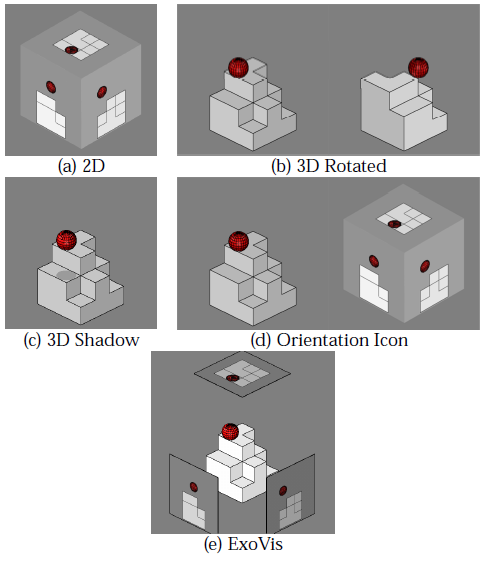
\includegraphics[width=0.5\linewidth]{./figures/tory06fig} 

}

\caption{Screen capture from
\textcite{tory_visualization_2006}: ``fig. 1 (a) 2D, (b) 3D Rotated, (c)
3D Shadow, (d) Orientation Icon, and (e) ExoVis displays used in
Experiment 1 (position estimation). Participants estimated the height of
the ball relative to the block shape. In this example, the ball is at
height 1.5 diameters above the block shape.''}\label{fig:tory06fig}
\end{figure}

\textcite{sedlmair_empirical_2013}, depicted in figure
\ref{fig:sedlmair13fig}, tasked users with cluster separation across 2D
scatterplot, 2D scatterplot matrices (SPLOMs) and interactive 3D
scatterplots as viewed in monocular 3D from a standard monitor. They
conclude that interactive 3D scatterplots perform worse for class
separation. This result is surprising as the extra dimension
theoretically allows for the clustering structure to be seen and
explored more clearly.














\begin{figure}

{\centering 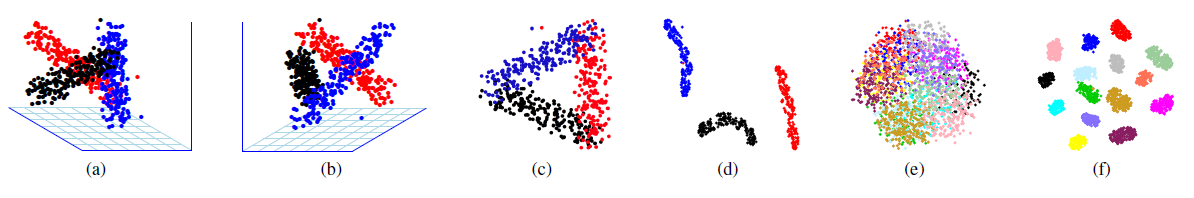
\includegraphics[width=1\linewidth]{./figures/sedlmair13fig} 

}

\caption{Screen capture of ``figure 5. Example of a mesh
display'' from \textcite{sedlmair_empirical_2013}: ``fig. 5. (a)-(d):
Screenshots of the entangled dataset \texttt{entangled1-3d-3cl-separate}
designed to show the most possible benefits for i3D. (a),(b) two
viewpoints of the same i3D PCA scatterplot. An accompanying video shows
the full 3D rotation. (c) 2D PCA projection. (d) t-SNE untangles this
class structure in 2D. (e)-(f): 2D scatterplots of the reduced
\texttt{entangled2-15d-adjacent} dataset which we designed to have a
ground truth entangled class structure in 15D. (e) Glimmer MDS cannot
untangle the classes, neither can PCA and robPCA (see supplemental
material). (f) t-SNE nicely untangles and separates the ground truth
classes in 2D.''}\label{fig:sedlmair13fig}
\end{figure}

\subsection{Comparing 3D and 2D embeddings of multivariate
data}\label{comparing-3d-and-2d-embeddings-of-multivariate-data}

\textcite{nelson_xgobi_1998}, depicted in figure \ref{fig:nelson98fig},
had \(n=15\) participants perform brushing and touring tasks
(identification of clusters, structure, and data dimensionality) in 3D
with head-tracked binocular VR. 3D proved to have a substantial
advantage for cluster identification and some advantage in identifying
the shape. Brushing did take longer in VR, perhaps due to the lower
familiarity of manipulating 3D spaces.







\begin{figure}

{\centering 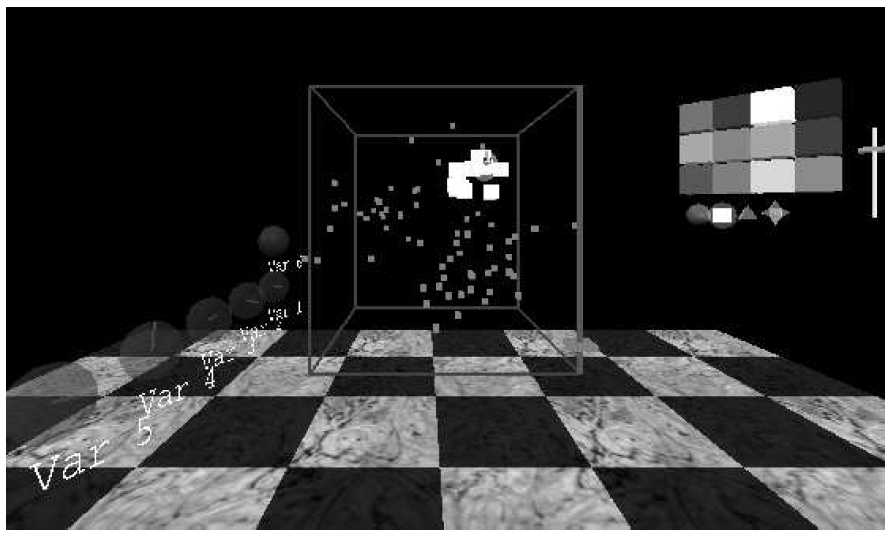
\includegraphics[width=0.7\linewidth]{./figures/nelson98fig} 

}

\caption{Screen capture from \textcite{nelson_xgobi_1998}:
``figure 4: This is a picture of a 3-D room, running VRGobi. Data is
plotted in the center, with painting tools to the right and variable
spheres to the left. In the viewing box, the data can be seen to contain
three clusters, and one is being brushed.''}\label{fig:nelson98fig}
\end{figure}

Another study, \textcite{gracia_new_2016} performed dimensionality
reduction down to 2- and 3D scatterplots, both displayed in monocular 3D
on a standard monitor. Users were found to more accurately compare
distances between points and identify outliers on 3D scatterplots.
However, both tasks were performed slower with the use of the 3D
scatterplots and statistical significance was not reported.

\textcite{wagner_filho_immersive_2018}, depicted in figure
\ref{fig:wagner18fig}, performed an \(n=30\) empirical study of PCA
embedded projections, and perception error across 4 tasks and 3 display
types: 2D, 3D, and immersive. Overall task error was less in 3D and
immersive relative to 2D. According to the user Likert-scale survey, 2D
is slightly easier to navigate and slightly more comfortable, while, 3D
and immersive display are slightly easier to interact and moderately
easier to find information.





\begin{figure}

{\centering 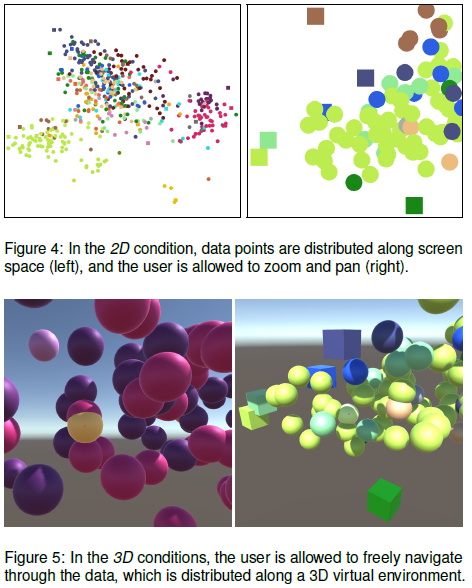
\includegraphics[width=0.5\linewidth]{./figures/wagner18fig} 

}

\caption{Screen capture from
\textcite{wagner_filho_immersive_2018}, original captions contained in
the capture.}\label{fig:wagner18fig}
\end{figure}

\subsection{Immersive analytics platform in
VR}\label{immersive-analytics-platform-in-vr}

Immersive analytics is an emerging field, where data visualization and
analysis is facilitated in an intuitive, immersive virtual reality
environment. An example of which is shown in
\textcite{cordeil_imaxes:_2017} introduces a collaborative space for
immersive data analysis. Where axes are displayed and intuitively
interacted with while responding to proximity to other variable axes and
popping into place changing the resulting geometric display. For
example, three variables can be placed as the \(x,~y,~z-\) axes for a 3D
scatterplot or stood up right next to each other for a parallel
coordinate plot. The subsequent work in
\textcite{cordeil_immersive_2019} builds from the previous reference and
refines it for the next iteration in interactive, scalable data
visualization in virtual spaces.




\begin{figure}

{\centering 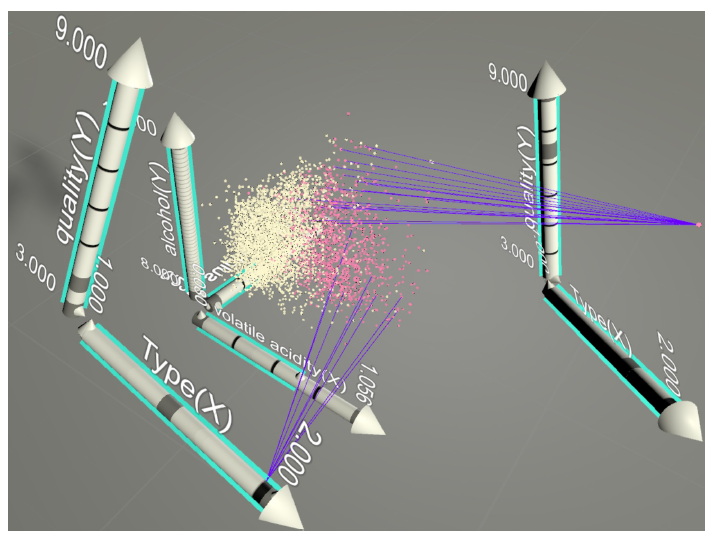
\includegraphics[width=0.5\linewidth]{./figures/cordeil2017fig} 

}

\caption{Screen capture of figure 15 from
\textcite{cordeil_imaxes:_2017}.}\label{fig:cordeil2017fig}
\end{figure}

\subsection{Research gaps}\label{research-gaps-1}

When comparing between 3D and 2D orthogonal views studies, in general,
show that perception accuracy is better in 3D, though manipulation speed
is generally slower. The speed discrepancy is confounded by the
difference in users familiar with manipulating 2D vs 3D spaces
\autocites{lee_effects_1986}{wickens_implications_1994}{tory_visualization_2006}[counterexample][]{sedlmair_empirical_2013}.

Similar results have been shown in static, 3D projected spaces
\autocites{gracia_new_2016}{wagner_filho_immersive_2018} and in dynamic
2D embedded spaces depicted in immersive 3D
\autocite{nelson_xgobi_1998}. With Modern VR hardware advancement, so
too does the quality, resolution, and prevalence of VR advance, making
VR more easily accessible than ever. It's time to view dynamic 3D
projections with immersive spaces and quantify the corresponding
benefits (\textbf{RO \#3 \& 4}).

\chapter{Work in progress}\label{ch:workinprogress}

Implementing UCS in low dimensions is fundamental to the extension of
the UCS into 3D space. The implementation of such forms the foundation
for future work addressed in the remaining research objectives.

\section{RO \#1) How can UCS be implemented in 1- and 2D
projections?}\label{ro-1-how-can-ucs-be-implemented-in-1--and-2d-projections}

This section covers the work done in the last year implementing USC via
\emph{manual tours}. Following experimental design methodology, this
work implements the manual tour as described in
\textcite{cook_manual_1997} and allows users to rotate a selected
variable into and out of a 2D projection of high-dimensional space for
user-controlled steering (UCS). The primary use is to determine the
sensitivity of the structure to the contributions of the manipulation
variable. This is particularly powerful for exploring the local
structure once a feature of interest has been identified by a guided
tour \autocite{cook_grand_1995} for example. The algorithm for a manual
tour allows rotations in horizontal, vertical, oblique, angular and
radial directions. In the algorithm below focuses on radial rotation.

Section \ref{sec:algorithm} explains the algorithm using a toy dataset.
A wider discussion of implementation as an \emph{R} package and
application to high energy physics data
\autocites{wang_visualizing_2018}{cook_dynamical_2018} is attached in
appendix \ref{ch:spinifex_paper} formatted as a paper that will be
submitted to The R Journal.

\section{Algorithm}\label{sec:algorithm}

Creating a manual tour animation requires these steps:

\begin{enumerate}
\def\labelenumi{\arabic{enumi}.}
\tightlist
\item
  Provided with a 2D projection, choose a variable to explore. This is
  called the ``manip'' variable.
\item
  Create a 3D manipulation space, where the manip variable has a full
  contribution.
\item
  Generate a rotation sequence which zeros coefficient and increases it
  to 1 before returning to the initial position.
\end{enumerate}

These steps are described in more detail below.

\subsection{Notation}\label{notation}

Start with multivariate data in an \(n \times p\) numeric matrix, and an
orthonormal \(d\)-dimensional basis set is describing the projection
from \(p-\) to \(d-\)space.

\begin{align*}
  \textbf{X}_{[n,~p]} ~=
  \begin{bmatrix}
    X_{1,~1} & \dots  & X_{1,~p} \\
    X_{2,~1} & \dots  & X_{2,~p} \\
    \vdots   & \ddots & \vdots   \\
    X_{n,~1} & \dots  & X_{n,~p}
  \end{bmatrix}
\end{align*}

\begin{align*}
  \textbf{B}_{[p,~d]} ~=
  \begin{bmatrix}
    B_{1,~1} & \dots  & B_{1,~d} \\
    B_{2,~1} & \dots  & B_{2,~d} \\
    \vdots   & \ddots & \vdots   \\
    B_{p,~1} & \dots  & B_{p,~d}
  \end{bmatrix}
\end{align*}

The algorithm is primarily operating on the projection basis and
utilizes the data only when making a display for computational
efficiency. A more comprehensive list of tour notation is given in
\ref{sec:tour_notation}.

\subsection{Toy data set}\label{toy-data-set}

The flea data from \textcite{lubischew_use_1962} will be used as an
example dataset. The data contains 74 observations across 6 variables,
corresponding to physical measurements of the insects. Each observation
belonging to one of three species.

A guided tour on the flea data is conducted by optimizing on the
\texttt{holes} index \autocite{cook_interactive_2007}. In a guided tour
the projection sequence is selected by optimizing an index of interest
in the projection. The \texttt{holes} index is maximized by when the
projected data has a lack of observations in the center. Figure
\ref{fig:step0}, shows an optimal projection of this data. The left plot
displays the projection basis, while the right plot shows the projected
data. The display of the basis has a unit circle with lines showing the
horizontal and vertical contributions of each variable in the
projection. Here is primarily \texttt{tars1} and \texttt{aede2}
contrasting the other four variables. In the projected data there are
three clusters, which have been colored, although not used in the
optimization. The question that will be explored in the explanation of
the algorithm is: how important is \texttt{aede2} to the separation of
the clusters.

\begin{figure}

{\centering 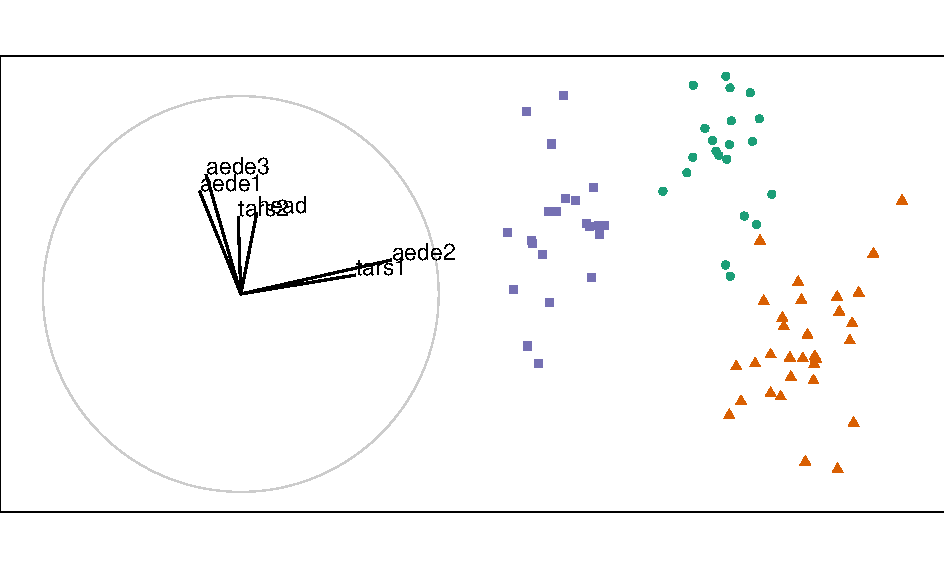
\includegraphics[width=0.98\linewidth]{confirmation_report_ns_files/figure-latex/step0-1} 

}

\caption{Basis reference frame (left) and projected data (right) of standardized flea data. Basis identified by holes-index guided tour. The variables `aede2` and `tars1` contribute mostly in the X direction, whereas the other variables contribute mostly in the Y direction. Select `aede2` as the manipulation variable to see how the structure of the projection changes.}\label{fig:step0}
\end{figure}

The left frame of figure \ref{fig:step0} shows the reference frame for
the basis. It describes the X and Y contributions of the basis as it
projects from the 6 variable dimensions down to 2. The right side shows
how the data looks projected through this basis. You can project a
single basis at any time through the matrix multiplication
\(\textbf{X}_{[n,~p]} ~*~ \textbf{B}_{[p,~d]} ~=~ \textbf{P}_{[n,~d]}\)
to such effect.

\subsection{Step 1 Choose variable of
interest}\label{step-1-choose-variable-of-interest}

Select a manipulation variable, \(k\). Initialize a zero vector \(e\)
and set the \(k\)-th element set to 1.

\begin{align*}
\textbf{e}_{[p,~1]} ~=~
  \begin{bmatrix}
    0 \\
    0 \\
    \vdots \\
    1 \\
    \vdots \\
    0
  \end{bmatrix}
\end{align*}

In figure \ref{fig:step0}, above, notice that the variables
\texttt{tars1} and \texttt{aede2} are almost orthogonal to the other 4
variables and control almost all of the variation in the x-axis of the
projection. \texttt{Aede2} has a larger contribution and is select it as
the manip variable.

\subsection{Step 2 Create the manip
space}\label{step-2-create-the-manip-space}

Use the Gram-Schmidt process to orthonormalize the concatenation of the
basis and \(e\) yielding the manip space.

\begin{align*}
  \textbf{M}_{[p,~d+1]}
  &= Orthonormalize_{GS}( \textbf{B}_{[p,~d]}|\textbf{e}_{[p,~1]} ) \\
  &= Orthonormalize_{GS}
  \left(
    \begin{bmatrix}
      B_{1,~1} & \dots  & B_{1,~d} \\
      B_{2,~1} & \dots  & B_{2,~d} \\
      \vdots   & \ddots & \vdots   \\
      B_{k,~1} & \dots  & B_{k,~d} \\
      \vdots   & \ddots & \vdots   \\
      B_{p,~1} & \dots  & B_{p,~d}
    \end{bmatrix}
  ~|~
    \begin{bmatrix}
      0 \\
      0 \\
      \vdots \\
      1 \\
      \vdots \\
      0
    \end{bmatrix}
  \right)
\end{align*}

Adding an extra dimension to our basis plane allows for the manipulation
of the specified variable. Orthonormalizing rescales the new vector
while leaving the first \(d\) variables identical to the basis. An
illustration of such can be seen below in figure \ref{fig:step2}.

\begin{figure}

{\centering 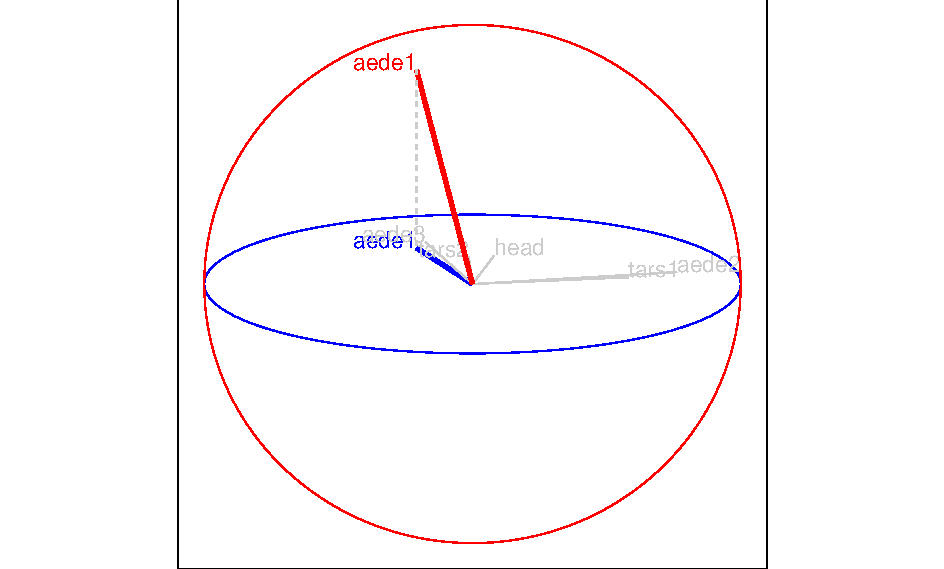
\includegraphics[width=1\linewidth]{confirmation_report_ns_files/figure-latex/step2-1} 

}

\caption{Manipulation space for controlling the contribution of aede2 of standardized flea data. Basis was identified by holes-index guided tour. The out of plane axis, in red, shows how the manipulation variable can be rotated, while other dimensions stay embedded within the basis plane.}\label{fig:step2}
\end{figure}

Imagine being able to grab hold of the red axis and rotate it changing
the projection onto the basis plane. This is what happens in a manual
tour. For a radial tour, fix \(\theta\), the angle within the blue
plane, and vary the \(\phi\), the angle orthogonal to the blue
projection plane. The user controlling these angles changes the values
of the coefficient the manip variable and performs a constrained
rotation on the remaining variables.

\subsection{Step 3 Generate rotation}\label{step-3-generate-rotation}

Define a set of values for \(\phi_i\), the angle of out of the plane
rotation, orthogonal to the projection plane. This corresponds to the
angle between the red manipulation axis and the blue plane in figure
\ref{fig:step2}.

\textbf{For } \(i\) \textbf{in 1 to n\_slides:}

For each \(\phi_i\), post multiply the manipulation space by a rotation
matrix, producing, \textbf{RM}, the rotated manip space.

\begin{align*}
  \textbf{RM}_{[p,~d+1,~i]}
  &= \textbf{M}_{[p,~d+1]} ~*~ \textbf{R}_{[d+1,~d+1]}
    ~~~~~~~~~~~~~~~~~~~~~~~~~~~~~~~~~~~~\text{For the $d=2$ case:} \\
  &= \begin{bmatrix}
    M_{1,~1} & \dots & M_{1,~d} & M_{1,~d+1} \\
    M_{2,~1} & \dots & M_{2,~d} & M_{2,~d+1} \\
    \vdots   & \ddots& \vdots   \\
    M_{p,~1} & \dots & M_{p,~d} & M_{p,~d+1}
  \end{bmatrix}_{[p,~d+1]}
    ~*~
  \begin{bmatrix}
    c_\theta^2 c_\phi s_\theta^2 &
    -c_\theta s_\theta (1 - c_\phi) &
    -c_\theta s_\phi \\
    -c_\theta s_\theta (1 - c_\phi) &
    s_\theta^2 c_\phi + c_\theta^2 &
    -s_\theta s_\phi \\
    c_\theta s_\phi &
    s_\theta s_\phi &
    c_\phi
  \end{bmatrix}_{[3,~3]}
\end{align*}

Where:

\begin{description}
  \item[$\theta$] is the angle that lies on the projection plane, the *XY*-scatterplot
  \item[$\phi$] is the angle orthogonal to the projection plane, in the *Z* direction relative to the *XY*-scatterplot
  \item[$c_\theta$] is the cosine of $\theta$
  \item[$c_\phi$]   is the cosine of $\phi$
  \item[$s_\theta$] is the sine of   $\theta$
  \item[$s_\phi$]   is the sine of   $\phi$
\end{description}

In application: compile the sequence of \(\phi_i\) and create an array
for each rotated manipulation space. \(\phi\) is the angle of change
relative to the \(\phi_1\), the transformation \(\phi_i\) - \(\phi_1\)
to useful to think about \(\phi\) relative to the basis plane. If the
manip variable doesn't move as expected this is the first place to
check.

Figure \ref{fig:step3} illustrates the sequence with 15 projected bases
and highlight the manip variable on top, while showing the corresponding
projected data points on the bottom. A dynamic version of this tour can
be viewed online at
\url{https://nspyrison.netlify.com/thesis/flea_manualtour_mvar5/}, (may
take a moment to load).








\begin{figure}

{\centering 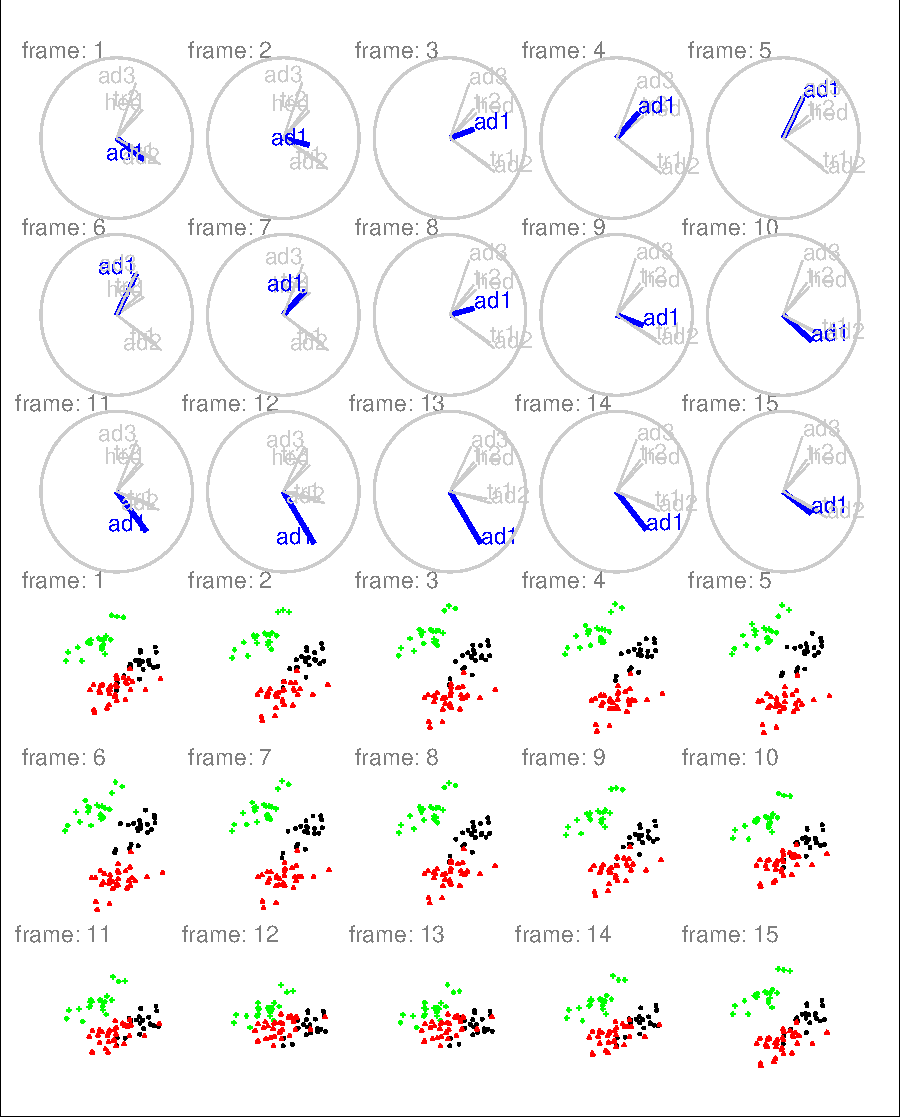
\includegraphics[width=6in,height=7.2in]{confirmation_report_ns_files/figure-latex/step3-1} 

}

\caption{Rotated manipulation spaces, a radial manual tour
manipulating \texttt{aded2} of standardized flea data. The manipulation
variable, \texttt{aede2}, extends from its initial contribution to a
full contribution to the projection before decreasing to zero, and then
returning to its initial state. A dynamic version can be viewed at
\url{https://nspyrison.netlify.com/thesis/flea_manualtour_mvar5/}.}\label{fig:step3}
\end{figure}

\section{Display projection sequence}\label{display-projection-sequence}

To get back to data-space pre-multiply the rotated manip space by the
data for the projection in data-space.

\begin{align}
  \textbf{P}_{[n,~d+1]}
    &= \textbf{X}_{[n,~p]} ~*~ \textbf{RM}_{[p,~d+1]} \\
    &=
      \begin{bmatrix}
          X_{1,~1} & \dots & X_{1,~p} \\
          X_{2,~1} & \dots & X_{2,~p} \\
          \vdots   & \vdots & \vdots  \\
          X_{n,~1} & \dots & X_{n,~p}
      \end{bmatrix}_{[n,~p]}
      ~*~
      \begin{bmatrix}
        RM_{1,~1} & RM_{1,~2} & RM_{1,~3} \\
        RM_{2,~1} & RM_{2,~2} & RM_{2,~3} \\
        \vdots    & \vdots    & \vdots    \\
        RM_{p,~1} & RM_{p,~2} & RM_{p,~3}
      \end{bmatrix}_{[p,~d+1]}
\end{align}

Plot the first \(d\) variables from each projection in sequence for an
\(XY\)-scatterplot. The remaining variable is sometimes linked to a data
point aesthetic to produce depth cues used in conjunction with the
\(XY\)-scatterplot.

\subsection{Storage and sharing}\label{storage-and-sharing}

Storing each data point for every frame with the overhead dynamic
graphics is very inefficient. In the same way that efficiency is gain by
performing math on the bases, the same approach suggested for storage
and sharing tours. Consider a radial manual tour, the salient features
can be stored in 3 bases, where \(\phi\) is at its starting, minimum,
and maximum values. The frames in between can be interpolated later by
supplying angular speed.

\chapter{Future work}\label{ch:future_work}

\section{RO \#2) Does 2D UCS provide benefits over
alternatives?}\label{ro-2-does-2d-ucs-provide-benefits-over-alternatives}

High dimensional data and models are ubiquitous but viewing them in data
space is not trivial. This work quantifies various measurements of 2D
UCS implemented in RO \#1, and commonly used alternatives. All
comparison groups are unsupervised (agnostic of clustering), static,
single embeddings in a lower dimension, and would include:

\begin{itemize}
\tightlist
\item
  \textbf{Principal Component Analysis (PCA)}, is a linear
  transformation that orients linear combinations of the variables into
  basis components and orders them according to the amount of variation.
  The first principal component is the linear combination that explains
  the most variation with the second explaining the most of the
  remaining variation and is orthogonal to all previous components, and
  so on.
\item
  \textbf{Multi-Dimensional Scaling (MDS)}, non-linear dimension
  reduction that compares pairwise distances between observations.
\item
  \textbf{t-distributed neighbor embeddings (tSNE)}, a nonlinear
  technique that iterates epochs of 1) constructing a probability
  distribution for selecting neighboring data and 2), minimizing
  Kullback-Leibler divergence (a measure of relative entropy).
\end{itemize}

Unfortunately, static linear projections necessarily cut variation in
the components not shown, while non-linear techniques lose transparency
back to the original variable space. Tours preserve this transparency to
variable-space and keep variation in tack. Providing user-controlled
steering of tours should allow for finer structural exploration than the
alternatives.

The methodology for this future work is a \textbf{case study} comparing
benchmark datasets across technique, UCS and leading alternatives. This
will be a sufficient comparison if there are enough quantifiable
measurements across the different techniques. However, if enough
measurements are not comparable across techniques an empirical study
analogous to the study suggested in RO \# 4 will be considered. Design
space includes data sets, techniques, and measures of comparison.

\section{RO \#3) How can UCS be extended to
3D?}\label{ro-3-how-can-ucs-be-extended-to-3d}

The literature has shown positive results for improved accuracy and
precision for 3D displays. Dynamic linear projections should have
similar gains in 2D projections, and the additional dimension should
allow for improved perception of surfaces and dynamic viewing of 3D
projections. The research answering RO \#1) will be extended to these
uses.

The work done in \textcite{cordeil_imaxes:_2017} creates a collaborative
space for people to engage in immersive data analysis, a generalized
platform for data visualization in the Unity game engine. By integrating
dynamic linear touring in 3D with the above work offers a consolidated
user interface that can be used across various display devices in RO
\#4.

This is an \textbf{algorithm design}, first, the \emph{R} package
spinifex will be extended to 3D and function projections will be
implemented. After the projections are performed \emph{Unity} will be
used to render the embeddings in 3D VR and offer a compatible front end
to be used across display devices.

Manipulating 3D spaces may not be straight forward. In section
\{sec:algorithm\} the manipulation space was in 3D, where 2 angles
defined a point that was projected back to the 2D projection. If we have
to define a 4D manipulation space it may be complex and clunky to
navigate. On the other hand, if we can control the projection to 3D with
the now 3D reference volume, then navigating 3D space may be very
intuitive.

Viewing functions and surfaces have several difficulties in 3D the first
of which is occulation, the surfaces in the foreground blocks the view
behind it. Opacity, wire mesh, and projection sectioning are ways to
address this issue. A second issue is that it may be disorienting or
nauseating to watch surfaces folding into each other.

If UCS happens in real time the angular speed of the tour should be
regulated for continuity of observation and to mitigate potentially
nauseating movement.

The design space includes the path generators (outlined in section
\ref{sec:path_generation}), geometric display (section
\ref{sec:geom_display}), layout in virtual space, dynamic interactions.
Tour paths are conceptually straight-forward mapping between values and
3D rendering. Each geometric display will need unique recreation, though
3D scatterplot, parallel coordinate plot and scatterplot matrices
(SPLOM) are currently supported in the respective packages in both
languages. We will also explore surface and function visualization in
3D.

\section{RO \#4) Does UCS in 3D displays provide perception benefits
over 2D displays?}\label{UCS_3dvs2d}

The bulk of past touring endeavors have existed whole in 2D, with the
exceptions of \textcite{nelson_xgobi_1998} and
\textcite{arms_benefits_1999} who performed an \(n=15\) experimental
study comparing tasks performed across 2D and 3D touring displays. The
XGobi interface was used on a standard 2D monitor while VRGobi (on the
C2 setup) was used with head-tracked binocular VR. The 3 accuracy tasks:
clustering, intrinsic data dimensionality, and radial sparseness were
recorded along with the speed of brushing data. Accuracy was the same
for the dimensionality task, while 3D display outperformed 2D on
clustering, and even more so on the radial sparsity. However, the time
taken to brush a cluster was less than half the time in 2D displays as
compared with 3D.

\textcite{wagner_filho_immersive_2018} performed a user study on the
perception of linear projections between 2D, 3D, and immersive 3D. The
\(n=30\) user study created 3D embeddings of multidimensional data via
principal component analysis (PCA, described in RO \#2, above). Users
performed 3 tasks across 2 data sets and 3 displays; 2D, 3D, and
immersive 3D. Data sets were chosen to have vastly different amounts of
information contained in the 3rd principal component. They find that the
introduction of a 3rd dimension in visualization improves task
performance (perception error, task error, and completion time)
regardless of immersion for only the dataset containing promising
information gain in 3D. Independent of the dataset, immersive 3D display
led to a larger subjective perception of accuracy and engagement.

The results of \textcite{wagner_filho_immersive_2018},
\textcite{nelson_xgobi_1998} and, \textcite{arms_benefits_1999} cast
positive light on 3D spaces improving the perception of embeddings of
high-dimensional data. Others have found the same for data already in
three dimensions. After implementing touring and UCS in 3D spaces (RO
\#3), the effects of viewing dynamic projections should be quantified
across the display type.

I plan to test the efficacy of doing so with the following controlled
\textbf{usability study}, where every participant will complete every
task on every display device. Task order and display device will be
randomly assigned to minimize learning bias. Correctness and speed of
tasks will be recorded alongside demographic data and subjective 5-point
Likert scale survey. A lineup-type model as outlined in
\textcite{hofmann_graphical_2012} may be employed to quantify the
``best'' display device.

Tasks will test the perception of structure and surface, varying across
the manipulation variable. All tasks will be conducted across at least
three display devices: standard 2D monitor, stereoscopic 3D monitor (on
a zSpace 200), and head-mounted VR goggles (HTC VIVE). The user
interface will be standardized across display devices. The data explored
will be of high energy physics experiments already being discussed in
publication \autocites{wang_visualizing_2018}{cook_dynamical_2018} and
looked at in 2D UCS in appendix \ref{ch:spinifex_paper}.

\chapter{PhD schedule}\label{ch:timeline}

\section{Timeline}\label{timeline}

\begin{center}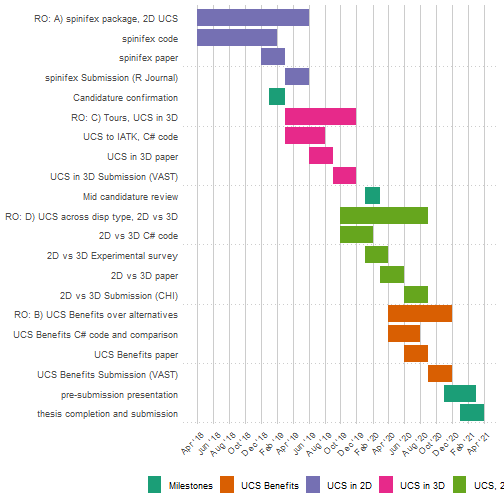
\includegraphics{confirmation_report_ns_files/figure-latex/timeline-1} \end{center}

\emph{Note RO \#2 logically would fit before RO \#3 \& 4 but is of lower
impact and retrospective case study. I move this research to the end to
give the other research objectives the priority.}

\section{Accompanying documents}\label{accompanying-documents}

\begin{itemize}
\tightlist
\item
  FIT 5144 hours

  \begin{itemize}
  \tightlist
  \item
    \textgreater{}120 hours \textbf{Tracked, awaiting mandatory events},
    due at the mid-candidature review
  \end{itemize}
\item
  WES Academic record

  \begin{itemize}
  \tightlist
  \item
    FIT6021: 2018 S2, \textbf{Completed} with Distinction
  \item
    FIT5144: 2019 S1+2, \textbf{Upcoming}, due at mid-candidature review
  \item
    FIT5113: 2018 S2, \textbf{Exemption submitted}, forwarded 14/02/2019
  \end{itemize}
\item
  myDevelopment - IT: Monash Doctoral Program - Compulsory Module

  \begin{itemize}
  \tightlist
  \item
    Monash Graduate Research Student Induction: \textbf{Completed}
  \item
    Research Integrity - Choose the Option most relevant:
    \textbf{Completed} (2 required of 4)
  \item
    Faculty Induction: \textbf{Content unavailable} (25/02/2019:
    ``Currently being updated and will be visible in this section
    soon'')
  \end{itemize}
\end{itemize}

\chapter{Source code}\label{sec:source}

This article was created in \texttt{R} \autocite{r_core_team_r:_2018},
using \texttt{bookdown} \autocite{xie_bookdown:_2016} and
\texttt{rmarkdown} \autocite{xie_r_2018}, with code generating the
examples inline.

Following good practice of version control and reproduction, the source
files can be found at
\href{https://github.com/nspyrison/Confirmation}{github.com/nspyrison/confirmation/}.

\appendix

\chapter{Glossary}\label{ch:glossary}

\section{Tour notation}\label{sec:tour_notation}

Terminology varies across articles. In my work, I use the following:

\begin{itemize}
\tightlist
\item
  \(n\), number of observations in the data.
\item
  \(p\), number of numeric variables, the dimensionality of data space.
\item
  \(d\), the dimensionality of projection space.
\item
  \(\textbf{X}_{[n,~p]}\), a data matrix in variable-space,
  \(\textbf{X} \in \mathbb{R}^{p}\). Typically centered, scaled, and
  optionally sphered.
\item
  \(\textbf{B}_{[p,~d]}\), orthonormal basis set (\(d\) linear
  combinations of \(p\) variables, each at a right angle, to the others,
  with a norm of 1), defining the axes directions for the projection
  from \(p-\) to \(d-\)space.
\item
  \(\textbf{Y}_{[n,~d]}\), projected data matrix in projection-space,
  \(\textbf{Y} \in \mathbb{R}^{d}\).
\item
  For projections down to 1- and 2D, it is common to display each
  variable contribution and direction on its axis (1D) or relative to a
  unit circle (2D), this is referred to as basis axes or sometimes the
  reference frame.
\item
  Geometric objects are referred to in generalized dimensions; the use
  of the term plane is not necessarily a 2D surface, but a hyperplane in
  the arbitrary dimensions of the projection space.
\end{itemize}

\section{Data visualization terminology}\label{sec:3d-terminology}

\begin{itemize}
\tightlist
\item
  2D - representation of data in 2 dimensions, without the use of depth
  perception cues and minimal aesthetic mapping (such as color, size,
  and height) to data points.
\item
  2.5D - Following the definition given in
  \textcite{ware_designing_2000}: visualizations that are essentially 2D
  but select depth cues are used to provide some suggestion of 3D.
  However, the term 2.5D is commonly used for several meanings \emph{due
  to the ambiguous use of 2.5D, this document errs on the side stating
  3D with descriptions of depth cues used}.
\item
  3D - visualizations of 3 dimensions with liberal use of depth cues
  unless otherwise qualified.
\item
  Depth perception cues - an indication that indicates the depth to an
  observer, including:

  \begin{itemize}
  \tightlist
  \item
    linear perspective - the property of parallel lines converging on a
    vanishing point.
  \item
    aerial perspective - objects that far away have lower contrast and
    color saturation due to light scattering in the atmosphere.
  \item
    occultation (or interposition) - where closer objects partially
    block the view of further objects.
  \item
    motion perspective/parallax - closer objects, move across the field
    of view faster than further objects.
  \item
    accommodation - the change of focal length due to change in the
    shape of the eye. Effective for distances of less than 2 meters.
  \item
    binocular stereopsis/disparity - the use of 2 images of slightly
    varied angles from the horizontal distance of the eyes. The
    disparity for distant objects is small, but it is significant for
    nearby objects.
  \item
    binocular convergence - The ocular-motor cue due to stereopsis
    focusing on the same objects. Convergence is effective for distances
    up to 10 meters.
  \end{itemize}
\item
  Virtual reality (VR) - a computer generated display of virtual spaces
  in place of physical vision.
\item
  Augmented reality (AR) - a computer generated display of information
  overlaid on a physical space.
\item
  Mixed reality (MR) - any degree of virtual or augmented reality.
\item
  Scatterplot matrices (SPLOM) - matrix display of pair-wise 2D
  scatterplots with 1D density on the diagonal.
\end{itemize}

\chapter{Using animation to explore sensitivity of structure in a
low-dimensional projection of high-dimensional data with user controlled
steering}\label{ch:spinifex_paper}

\emph{The content contained in this appendix document is work done in
the last year of my research and currently formatted as a paper to be
submitted to the R Journal.}

\section{Abstract}\label{abstract-1}

The tour algorithm, and its various versions provide a systematic
approach to viewing low-dimensional projections of high-dimensional
data. It is particularly useful for understanding multivariate data, and
useful in association with techniques for dimension reduction,
supervised and unsupervised classification. The \emph{R} package
\emph{tourr} provides many methods for conducting tours on multivariate
data. This paper discusses an extension package which adds support for
the manual tour, called \emph{spinifex}. It is particularly usefully for
exploring the sensitivity of structure discovered in a projection by a
guided tour, to the contribution of a variable. \emph{Spinifex} utilizes
the animation packages \emph{plotly} and \emph{gganimation} to allow
users to rotate the selected variable into and out of a chosen
projection.

Keywords: grand tour, projection pursuit, manual tour, high dimensional
data, multivariate data, data visualization, statistical graphics, data
science, data mining.

\section{Introduction}\label{introduction}

A tour is a multivariate data analysis technique in which is a sequence
of linear (orthogonal) projections into a lower subspace in which
\(p-\)space is rotated across time. Each frame of the sequence
corresponds to a small change in the projection for a smooth transition
to persevere the object continuity.

Multivariate data analysis can be broken into 2 groups: linear and
non-linear transformations. Like PCA and LDA, touring uses linear
dimension reduction that maintain transparency back to the original
variable-space. PCA and LDA are typically represented with single static
projection as a 2- or 3D scatterplot, inherently losing the variation
held with the high components, whereas touring keeps the information in
tack by showing the other components across time. Non-linear
transformations such as tSNE (t-distributed stochastic nearest neighbor
embeddings), MDS (multi-dimension scaling), and LLE (local linear
embedding) distort the parameter-space which lacks transparency back to
the original parameter-space. They show more extreme separation in
embeddings, but the variable opacity can be a non-starter for many uses.

There are many ways that a tour path can be generated, we will focus on
one, the manual tour. The manual tour was described in
\textcite{cook_manual_1997} and allows a user to rotate a variable into
and out of a 2D projection of high-dimensional space. This will be
called user-controlled steering (UCS). The primary purpose is to
determine the sensitivity of structure visible in a projection to the
contributions of a variable. Manual touring can also be useful for
exploring the local structure once a feature of interest has been
identified, for example, by a guided tour \autocite{cook_grand_1995}.
The algorithm for a manual tour allows rotations in horizontal,
vertical, oblique, angular and radial directions. Rotation in a radial
direction, would pull a variable into and out of the projection, which
allows for examining the sensitivity of structure in the projection to
the contribution of this variable. This type of manual rotation is the
focus of this paper.

A manual tour relies on user input, and thus has been difficult to
program in R. Ideally, the mouse movements of the user are captured, and
passed to the computations, driving the rotation interactively. However,
this type of interactivity is not simple in R. This has been the reason
that the algorithm was not incorporated into the \emph{tourr} package.
Spinifex utilizes two new animation packages, \emph{plotly}
\autocite{sievert_plotly_2018} and \emph{gganimate}
\autocite{pedersen_gganimate:_2019}, to display manual tours or other
saved tours. From a given projection, the user can choose which variable
to control, and the animation sequence is generated to remove the
variable from the projection, and then extend its contribution to be the
sole variable in one direction. This allows the viewer to assess the
change in structure induced in the projection by the variable's
contribution.

The paper is organized as follows. Section \ref{sec:algorithm} explains
the algorithm using a toy dataset. Section \ref{sec:application}
illustrates how this can be used for sensitivity analysis. The last
section, \ref{sec:discussion_paper} summarizes the work and discusses
future research.

\section{Algorithm}\label{sec:algorithm_paper}

Creating a manual tour animation requires these steps:

\begin{enumerate}
\def\labelenumi{\arabic{enumi}.}
\tightlist
\item
  Provided with a 2D projection, choose a variable to explore. This is
  called the ``manip'' variable.
\item
  Create a 3D manipulation space, where the manip variable has full
  contribution.
\item
  Generate a rotation sequence which zero's the norm of the coefficient
  and increases it to 1.
\end{enumerate}

These steps are described in more detail below.

\subsection{Notation}\label{notation-1}

This section describes the notation used in the algorithm description.
The data to be displayed is an \(n \times p\) numeric matrix.

\begin{align*}
  \textbf{X}_{[n,~p]} ~=
  \begin{bmatrix}
    X_{1,~1} & \dots  & X_{1,~p} \\
    X_{2,~1} & \dots  & X_{2,~p} \\
    \vdots   & \ddots & \vdots   \\
    X_{n,~1} & \dots  & X_{n,~p}
  \end{bmatrix}
\end{align*}

An orthonormal \(d\)-dimensional basis set is describing the projection
from \(p-\) to \(d-\) space

\begin{align*}
  \textbf{B}_{[p,~d]} ~=
  \begin{bmatrix}
    B_{1,~1} & \dots  & B_{1,~d} \\
    B_{2,~1} & \dots  & B_{2,~d} \\
    \vdots   & \ddots & \vdots   \\
    B_{p,~1} & \dots  & B_{p,~d}
  \end{bmatrix}
\end{align*}

The algorithm is primarily operating on the projection basis and
utilizes the data only when making a display.

\subsection{Toy data set}\label{toy-data-set-1}

The flea data from the R package \emph{tourr}
\autocite{wickham_tourr_2011}, is used to illustrate the algorithm. The
data, originally from \textcite{lubischew_use_1962}, contains 74
observations across 6 variables, which physical measurements of the
insects. Each observation belonging to one of three species.

A guided tour on the flea data is conducted by optimizing on the
\texttt{holes} index \autocite{cook_interactive_2007}. In a guided tour
the data the projection sequence is shown by optimizing an index of
interest. The holes index is maximized by when the projected data has a
lack of observations in the center. Figure \ref{fig:step0}, shows an
optimal projection of this data. The left plot displays the projection
basis, while the right plot shows the projected data. The display of the
basis has a unit circle with lines showing the horizontal and vertical
contributions of each variable in the projection. Here is primarily
tars1 and aede2 contrasting the other four variables. In the projected
data there are three clusters, which have been colored, although not
used in the optimization. The question that will be explored in the
explanation of the algorithm is how important is aede2 to the separation
of the clusters.

\begin{figure}

{\centering \includegraphics[width=0.98\linewidth]{confirmation_report_ns_files/figure-latex/step0-paper-1} 

}

\caption{Basis reference frame (left) and projected data (right) of standardized flea data. Basis identified by holes-index guided tour. The variables `aede2` and `tars1` contribute mostly in the x direction, whereas the other variables contribute mostly in the y direction. We'll select `aede2` as our manipulation variable to see how the structure of the projection changes as we rotate `aede2` into and out of the projection.}\label{fig:step0-paper}
\end{figure}

The left frame of figure \ref{fig:step0-paper} shows the reference frame
for the basis. It describes the X and Y contributions of the basis as it
projects from the 6 variable dimensions down to 2. Call
\texttt{view\_basis()} on a basis to produce a similar image as a
\texttt{ggplot2} object. The right side shows how the data looks
projected through this basis. You can project a single basis at any time
through the matrix multiplication
\(\textbf{X}_{[n,~p]} ~*~ \textbf{B}_{[p,~d]} ~=~ \textbf{P}_{d[n,~d]}\)
to such effect.

\subsection{Step 1 Choose variable of
interest}\label{step-1-choose-variable-of-interest-1}

Select a manipulation variable, \(k\). Initialize a zero vector \(e\)
and set the \(k\)-th element set to 1.

\begin{align*}
\textbf{e}_{[p,~1]} ~=~
  \begin{bmatrix}
    0 \\
    0 \\
    \vdots \\
    1 \\
    \vdots \\
    0
  \end{bmatrix}
\end{align*}

In figure \ref{fig:step0-paper}, above, notice that the variables
\texttt{tars1} and \texttt{aede2} are almost orthogonal to the other 4
variables and control almost all of the variation in the x axis of the
projection. \texttt{Aede2} has a larger contribution in this basis, so
we'll select it as the manip variable.

\subsection{Step 2 Create the manip
space}\label{step-2-create-the-manip-space-1}

Use the Gram-Schmidt process to orthonormalize the concatenation of the
basis and \(e\) yielding the manipulation space.

\begin{align*}
  \textbf{M}_{[p,~d+1]}
  &= Orthonormalize_{GS}( \textbf{B}_{[p,~d]}|\textbf{e}_{[p,~1]} ) \\
  &= Orthonormalize_{GS}
  \left(
    \begin{bmatrix}
      B_{1,~1} & \dots  & B_{1,~d} \\
      B_{2,~1} & \dots  & B_{2,~d} \\
      \vdots   & \ddots & \vdots   \\
      B_{k,~1} & \dots  & B_{k,~d} \\
      \vdots   & \ddots & \vdots   \\
      B_{p,~1} & \dots  & B_{p,~d}
    \end{bmatrix}
  ~|~
    \begin{bmatrix}
      0 \\
      0 \\
      \vdots \\
      1 \\
      \vdots \\
      0
    \end{bmatrix}
  \right)
\end{align*}

In R it looks like the below chunk. \texttt{tourr::orthonormalise()}
uses the Gram Schmidt process (rather than Householder reflection) to
orthonormalize.

\begin{Shaded}
\begin{Highlighting}[]
\NormalTok{  e            <-}\StringTok{ }\KeywordTok{rep}\NormalTok{(}\DecValTok{0}\NormalTok{, }\DataTypeTok{len =} \KeywordTok{nrow}\NormalTok{(basis))}
\NormalTok{  e[manip_var] <-}\StringTok{ }\DecValTok{1}
\NormalTok{  manip_space  <-}\StringTok{ }\NormalTok{tourr}\OperatorTok{::}\KeywordTok{orthonormalise}\NormalTok{(}\KeywordTok{cbind}\NormalTok{(basis, e))}
\end{Highlighting}
\end{Shaded}

Adding an extra dimension to our basis plane allows for the manipulation
of the specified variable. Orthonormalizing rescales the new vector,
while leaving the first \(d\) variables identical to the basis. An
illustration of such can been seen below in figure
\ref{fig:step2-paper}.

\begin{figure}

{\centering \includegraphics[width=1\linewidth]{confirmation_report_ns_files/figure-latex/step2-paper-1} 

}

\caption{Manipulation space for controlling the contribution of aede2 of standardized flea data. Basis was identified by holes-index guided tour. The out of plane axis, in red, shows how the manipulation variable can be rotated, while other dimensions stay embedded within the basis plane.}\label{fig:step2-paper}
\end{figure}

Imagine being able to grab hold of the red axis and rotate it changing
the projection onto the basis plane. This is what happens in a manual
tour. For a radial tour we fix, \(\phi\), the angle within the blue
plain, and vary the \(\theta\), the angle between the red and blue
lines. The user controlling these angles changes the values of the
coefficient the manip variable and performs a constrained rotation on
the remaining variables.

\subsection{Step 3 Generate rotation}\label{step-3-generate-rotation-1}

Define a set of values for \(\phi_i\), the angle of out of plane
rotation, orthogonal to the projection plane. This corresponds to the
angle between the red manipulation axis and the blue plane in figure
\ref{fig:step2-paper}.

\textbf{For } \(i\) \textbf{in 1 to n\_slides:}

For each \(\phi_i\), post multiply the manipulation space by a rotation
matrix, producing, \textbf{RM}, the rotated manip space.

\begin{align*}
  \textbf{RM}_{[p,~d+1,~i]}
  &= \textbf{M}_{[p,~d+1]} ~*~ \textbf{R}_{[d+1,~d+1]}
    ~~~~~~~~~~~~~~~~~~~~~~~~\text{For the $d=2$ case:} \\
  &= \begin{bmatrix}
    M_{1,~1} & \dots & M_{1,~d} & M_{1,~d+1} \\
    M_{2,~1} & \dots & M_{2,~d} & M_{2,~d+1} \\
    \vdots   & \ddots& \vdots   \\
    M_{p,~1} & \dots & M_{p,~d} & M_{p,~d+1}
  \end{bmatrix}_{[p,~d+1]}
    ~*~
  \begin{bmatrix}
    c_\theta^2 c_\phi s_\theta^2 &
    -c_\theta s_\theta (1 - c_\phi) &
    -c_\theta s_\phi \\
    -c_\theta s_\theta (1 - c_\phi) &
    s_\theta^2 c_\phi + c_\theta^2 &
    -s_\theta s_\phi \\
    c_\theta s_\phi &
    s_\theta s_\phi &
    c_\phi
  \end{bmatrix}_{[3,~3]}
\end{align*}

Where:

\begin{description}
  \item[$\theta$] is the angle that lies on the projection plane, the *XY*-scatterplot
  \item[$\phi$] is the angle orthogonal to the projection plane, in the *Z* direction relative to the *XY*-scatterplot
  \item[$c_\theta$] is the cosine of $\theta$
  \item[$c_\phi$]   is the cosine of $\phi$
  \item[$s_\theta$] is the sine of   $\theta$
  \item[$s_\phi$]   is the sine of   $\phi$
\end{description}

In application: compile the sequence of \(\phi_i\) and create an array
(or long table) for each rotated manipulation space. \(\phi\) is the
angle relative to the \(\phi_1\), we find the transformation \(\phi_i\)
- \(\phi_1\) useful to think about \(\phi\) relative to the basis plane.
If the manip variable doesn't move as expected this is the first place
to check.

\begin{Shaded}
\begin{Highlighting}[]
\ControlFlowTok{for}\NormalTok{ (phi }\ControlFlowTok{in} \KeywordTok{seq}\NormalTok{(seq_start, seq_end, phi_inc_sign)) \{}
\NormalTok{  slide <-}\StringTok{ }\NormalTok{slide }\OperatorTok{+}\StringTok{ }\DecValTok{1}
\NormalTok{  tour[,, slide] <-}\StringTok{ }\KeywordTok{rotate_manip_space}\NormalTok{(manip_space, theta, phi)[, }\DecValTok{1}\OperatorTok{:}\DecValTok{2}\NormalTok{]}
\NormalTok{\}}
\end{Highlighting}
\end{Shaded}

In figure \ref{fig:step3-paper} we illustrate the sequence with 15
projected bases and highlight the manip variable on top, while showing
the corresponding projected data points on the bottom. A dynamic version
of this tour can be viewed online at
\url{https://nspyrison.netlify.com/thesis/flea_manualtour_mvar5/}, will
take a moment to load. This format of this figure and linking to dynamic
version will be used again in section \ref{sec:application}.









\begin{figure}

{\centering \includegraphics[width=6in,height=7.2in]{confirmation_report_ns_files/figure-latex/step3-paper-1} 

}

\caption{Rotated manipulation spaces, a radial manual tour
controlling the contribution from \texttt{aded2} of standardized flea
data. The contribution of \texttt{aede2} extends from its initial
contribution to a full contribution to the projection before decreasing
to zero, and then returning to its initial state. A dynamic version can
be viewed at
\url{https://nspyrison.netlify.com/thesis/flea_manualtour_mvar5/}.}\label{fig:step3-paper}
\end{figure}

\section{Display projection
sequence}\label{display-projection-sequence-1}

To get back to data-space pre-multiply the rotated manip space by the
data for the projection in data-space.

\begin{align}
  \textbf{P}_{[n,~d+1]}
    &= \textbf{X}_{[n,~p]} ~*~ \textbf{RM}_{[p,~d+1]} \\
    &=
      \begin{bmatrix}
          X_{1,~1} & \dots & X_{1,~p} \\
          X_{2,~1} & \dots & X_{2,~p} \\
          \vdots   & \vdots & \vdots  \\
          X_{n,~1} & \dots & X_{n,~p}
      \end{bmatrix}_{[n,~p]}
      ~*~
      \begin{bmatrix}
        RM_{1,~1} & RM_{1,~2} & RM_{1,~3} \\
        RM_{2,~1} & RM_{2,~2} & RM_{2,~3} \\
        \vdots     & \vdots     & \vdots     \\
        RM_{p,~1} & RM_{p,~2} & RM_{p,~3}
      \end{bmatrix}_{[p,~d+1]}
\end{align}

Plot the first 2 variables from each projection in sequence for an XY
scatterplot. The remaining variable is sometimes linked to a data point
aesthetic to produce depth cues used in conjunction with the XY
scatterplot.

\emph{tourr} utilizes R's base graphics for the display of tours. Use
\texttt{render\_plotly()} to display as an dynamic \texttt{plotly}
\textcite{sievert_plotly_2018} object or \texttt{render\_gganimate()}
for a \texttt{gganimate} \textcite{pedersen_gganimate:_2019} graphic. A
third notable animation related package is \texttt{animation}
\textcite{xie_animation:_2018}. It's not yet implemented in
\texttt{spinifex} as it uses base graphics, whereas the former two are
compatible with \texttt{ggplot2}.

Interaction with graphics in R is limited. Traditionally, all commands
are passed to the R via calls to the console, conflicting with user
engagement. Some recent packages have made advancement into this
direction such as with the use of the R package \texttt{shinny}, which
custom-made applications can be hosted either locally or remotely and
interact with the R console, allowing for developers to code dynamic
content interaction. To a lesser extent \texttt{plotly} offers static
interactions with contained object, such as tool tips, brushing, and
linking without communicating back to the R console.

\subsection{Storage and sharing}\label{storage-and-sharing-1}

Storing each data point for every frame with the overhead dynamic
graphics is very inefficient. In the same way that we gain efficiency by
performing math on the bases, that is the same approach suggested for
storage and sharing tours. Consider a radial manual tour, we can store
the salient features in 3 bases, where \(\phi\) is at its starting,
minimum, and maximum values. The frames in between can be interpolated
by supplying angular speed. By using the \texttt{tourr::save\_history()}
we can do just that. Save such tour path history and a single set of the
data offers a performant storage and transferring.

\section{Application}\label{sec:application}

In a recent paper, \textcite{wang_visualizing_2018}, the authors
aggregate and visualize the sensitivity of hadronic experiments. The
authors introduce a new tool, PDFSense, to aid in the visualization of
parton distribution functions (PDF). The parameter-space of these
experiments lies in 56 dimensions, \(\delta \in \mathbb{R}^{56}\), and
are presented in this work in 3D subspaces of the 10 first principal
components and non-linear embeddings.

The work in \textcite{cook_dynamical_2018} applies touring for discern
finer structure of this sensitivity. Table 1 of Cook et. al. summaries
the key findings of PDFSense \& TFEP (TensorFlow embedded projection)
and those from touring. The authors selected the 6 first principal
components, containing 48\% of the variation held within the full data
when centered, but not sphered. This data contained 3 clusters: jet,
DIS, and VBP. Below pick up from the projections used in their figures 7
and 8 (jet and DIS clusters respectively) and apply manual tours to
explore the local structure with finer precision.

\subsection{Jet cluster}\label{jet-cluster}

The jet cluster is of particular interest as it contains the largest
data sets and is found to be important in
\textcite{wang_visualizing_2018}. The jet cluster resides in a smaller
dimensionality than the full set of experiments with 4 principal
components explaining 95\% of its variation
\autocite{cook_dynamical_2018}. We subset the data down to ATLAS7old and
ATLAS7new to narrow in on 2 groups with a reasonable number of
observations and occupy different parts of the subspace. Below, we
perform radial manual tours on various principal components within this
scope. In PC3 and PC4 are manipulated in figure \ref{fig:JetClusterGood}
and figure \ref{fig:JetClusterBad} respectively. Manipulating PC3, where
varying the angle of rotation brings interesting features in-to and out
of the center mass of the data, is interesting than the manipulation of
PC4, where features are mostly independent of the manip var.










\begin{figure}

{\centering 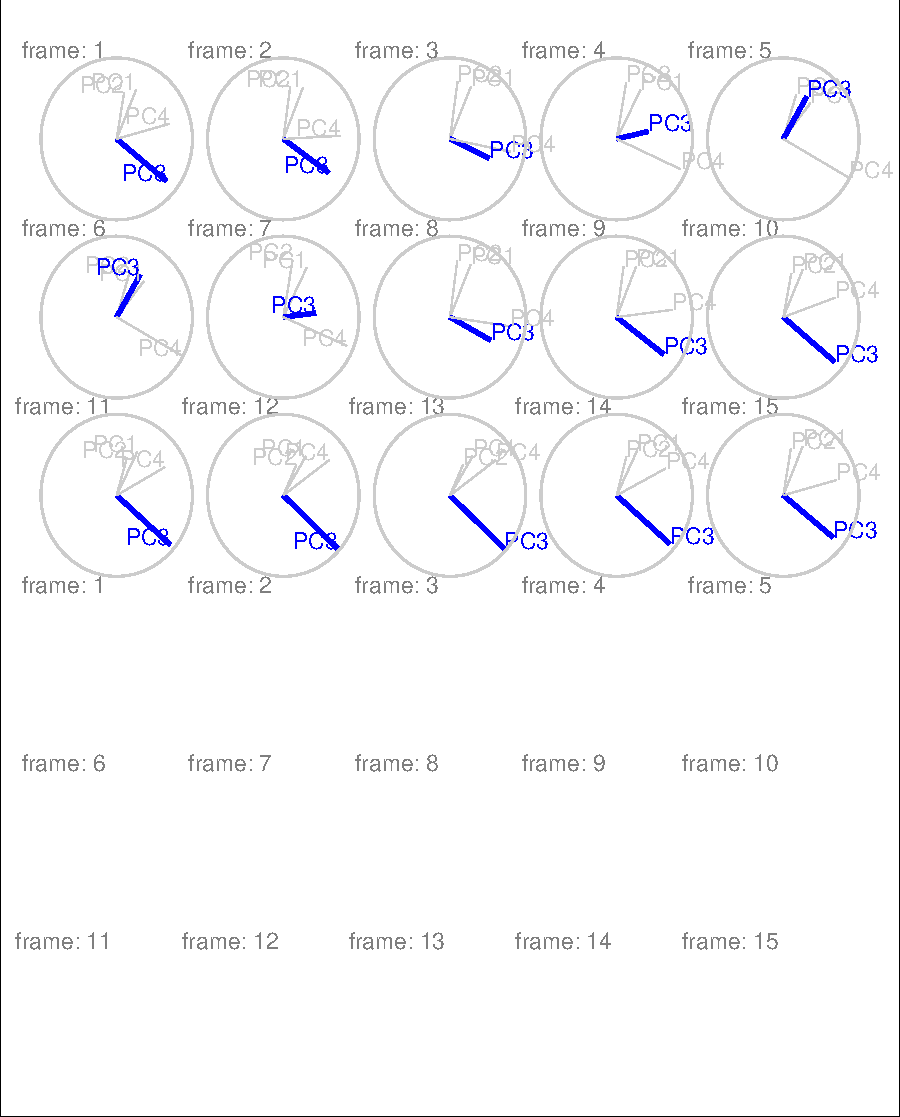
\includegraphics[width=6in,height=7.2in]{confirmation_report_ns_files/figure-latex/JetClusterGood-1} 

}

\caption{Jet cluster, radial manual tour of PC3. Colored
by experiment type: `ATLAS7new' in green and `ATLAS7old' in orange. When
PC3 fully contributes to the projection ATLAS7new (green) occupies
unique space and several outliers are identifiable. Zeroing the
contribution from PC3 to the projection hides the outliers and indeed
all observations with ATLAS7new are contained within ATLAS7old (orange).
A dynamic version can be viewed at
\url{https://nspyrison.netlify.com/thesis/jetcluster_manualtour_pc3/}.}\label{fig:JetClusterGood}
\end{figure}









\begin{figure}

{\centering 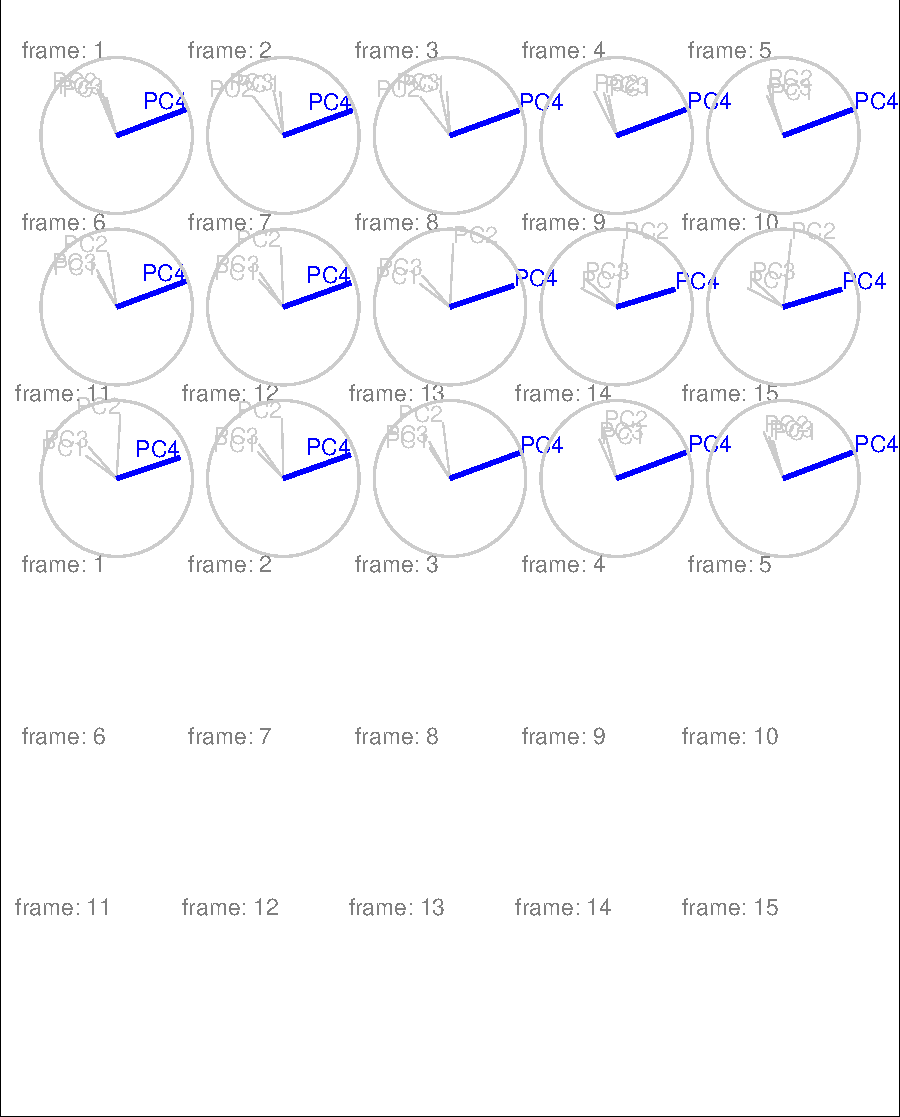
\includegraphics[width=6in,height=7.2in]{confirmation_report_ns_files/figure-latex/JetClusterBad-1} 

}

\caption{Jet cluster, radial manual tour of PC4. Colored
by experiment type: `ATLAS7new' in green and `ATLAS7old' in orange. This
tour contains less interesting information ATLAS7new (green) has points
that are right and left of ATLAS7old, while most points occupy the same
projection space, regardless of the contribution of PC4. A dynamic
version can be viewed at
\url{https://nspyrison.netlify.com/thesis/jetcluster_manualtour_pc3/}.}\label{fig:JetClusterBad}
\end{figure}

Jet cluster manual tours manipulating each of the principal components
can be viewed from the links:
\href{https://nspyrison.netlify.com/thesis/jetcluster_manualtour_pc1/}{PC1},
\href{https://nspyrison.netlify.com/thesis/jetcluster_manualtour_pc2/}{PC2},
\href{https://nspyrison.netlify.com/thesis/jetcluster_manualtour_pc3/}{PC3},
and
\href{https://nspyrison.netlify.com/thesis/jetcluster_manualtour_pc4/}{PC4}.

\subsection{DIS cluster}\label{dis-cluster}

We perform a manual tour on this data, manipulating PC6 as depicted in
figure \ref{fig:DISclusterGood}. Looking at several frames we see that
DIS HERA lie mostly on a plane. When PC6 has full contributions, we see
the dimuon SIDIS in purple is almost orthogonal to the DIS HERA (green).
Yet the contribution of PC6 is zeroed the dimuon SIDIS data occupy the
same space as the DIS HERA data. A dynamic version of this manual tour
can be found at:
\url{https://nspyrison.netlify.com/thesis/discluster_manualtour_pc6/}.
The page takes a bit to load, as the animation is several megabytes.











\begin{figure}

{\centering 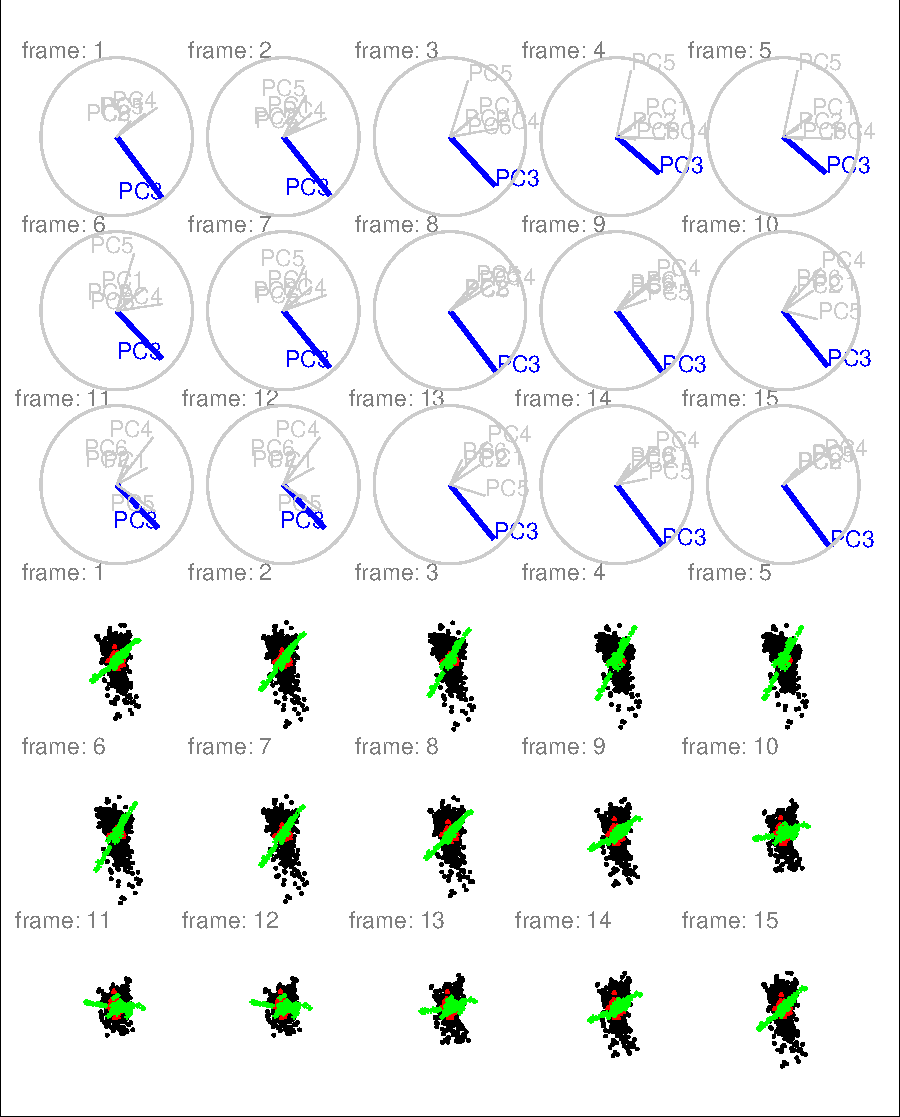
\includegraphics[width=6in,height=7.2in]{confirmation_report_ns_files/figure-latex/DISclusterGood-1} 

}

\caption{DIS cluster, radial manual tour of PC6. colored
by experiment type: `DIS HERA1+2' in green, `dimuon SIDIS' in purple,
and `charm SIDIS' in orange. When the contribution PC 6 is large we see
that dimuon SIDIS (purple) data are nearly orthogonal to DIS HERA
(green) data. As the data is rotated, we can also see that DIS HERA
(green) practically lie on a plane in this 6-d subspace. When the
contribution of PC6 is near zero, dimonSIDIS (purple) occupies the same
space as the DIS HERA data. A dynamic version can be viewed at
\url{https://nspyrison.netlify.com/thesis/discluster_manualtour_pc6/}.}\label{fig:DISclusterGood}
\end{figure}

This is different story than if we had selected a different variable to
manipulate. In figure \ref{fig:DISclusterBad} we manipulate PC2.










\begin{figure}

{\centering 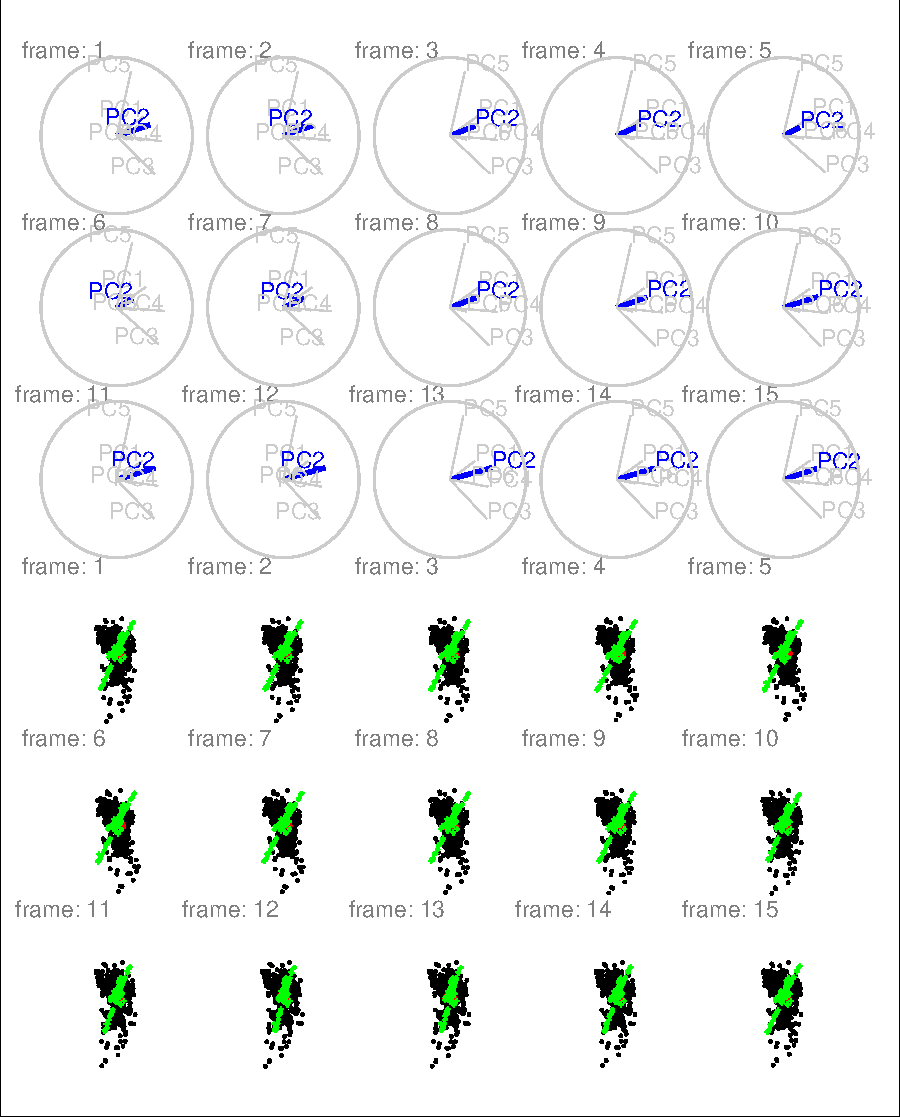
\includegraphics[width=6in,height=7.2in]{confirmation_report_ns_files/figure-latex/DISclusterBad-1} 

}

\caption{DIS cluster, radial manual tour of PC2. Colored
by experiment type: `DIS HERA1+2' in green, `dimuon SIDIS' in purple,
and `charm SIDIS' in orange. The structure of previously described plane
of DIS HERA (green) and nearly orthogonal dimuon SIDIS (purple) is
present, however the manipulating PC2 does not give a head-on view of
either, a less useful manual tour than that of PC6. A dynamic version
can be viewed at
\url{https://nspyrison.netlify.com/thesis/discluster_manualtour_pc2/}.}\label{fig:DISclusterBad}
\end{figure}

DIS cluster manual tours manipulating each of the principal components
can be viewed from the links:
\href{https://nspyrison.netlify.com/thesis/discluster_manualtour_pc1/}{PC1},
\href{https://nspyrison.netlify.com/thesis/discluster_manualtour_pc2/}{PC2},
\href{https://nspyrison.netlify.com/thesis/discluster_manualtour_pc3/}{PC3},
\href{https://nspyrison.netlify.com/thesis/discluster_manualtour_pc4/}{PC4},
\href{https://nspyrison.netlify.com/thesis/discluster_manualtour_pc5/}{PC5},
and
\href{https://nspyrison.netlify.com/thesis/discluster_manualtour_pc6/}{PC6}.

\section{Source code and usage}\label{source-code-and-usage}

This article was created in \texttt{R} \autocite{r_core_team_r:_2018},
using \texttt{bookdown} \autocite{xie_bookdown:_2016} and
\texttt{rmarkdown} \autocite{xie_r_2018}, with code generating the
examples inline. The source files can be found at:
\href{https://github.com/nspyrison/confirmation/}{github.com/nspyrison/confirmation/}.

The source code for the \texttt{spinifex} package can be found at
\href{https://github.com/nspyrison/spinifex/}{github.com/nspyrison/spinifex/}.
To install the package in R, run:

\begin{Shaded}
\begin{Highlighting}[]
\CommentTok{# install.package("devtools")}
\NormalTok{devtools}\OperatorTok{::}\KeywordTok{install_github}\NormalTok{(}\StringTok{"nspyrison/spinifex"}\NormalTok{)}
\end{Highlighting}
\end{Shaded}

\section{Discussion}\label{sec:discussion_paper}

This work has described an algorithm and package for exploring
conducting a manual tour, from a 2D projection, to explore the
sensitivity of structure to the contributions of a variable.

Future work on the algorithm and package would include developing it to
work with arbitrary projection dimension, enabling the method to operate
on other displays like parallel coordinates, and implementing the
unconstrained manual control, called oblique in
\textcite{cook_manual_1997}.

The Givens rotations and Householder reflections as outlined in
\textcite{buja_computational_2005} may provide a way to conduct higher
dimensional manual control. In a Givens rotation, the \(x\) and \(y\)
components (for example \(\theta~= 0,~pi/2\)) of the in-plane rotation
are calculated separately and would be applied sequentially to produce
the radial rotation. Householder reflections define reflection axes to
project points on to the axes and generate rotations.

The \emph{tourr} package provides several \(d\)-dimensional graphic
displays including Andrews curves, Chernoff faces, parallel coordinate
plots, scatterplot matrix, and radial glyphs. Having manual controls
available for these types of displays would require a
dimensionally-generalized rotation matrix.

Development of a graphical user interface, e.g. \emph{shiny} app, would
make the \emph{spinifex} package more flexible. The user could easily
switch between variables to control, adjust the step size to make
smoother rotation sequences, or save any state to continue to continue
to explore the contributions of other variables.

\printbibliography[heading=bibintoc]



\end{document}
